\def\coursename{量子力学}
\def\courseEnglishname{Quantum Mechanics}
\def\teachername{陈新老师、郭永}
\def\beginday{2022/3/25}

\documentclass[a4paper, 11pt]{article}

\usepackage[UTF8]{ctex}

\usepackage[T1]{fontenc}								% 字体
\catcode`\。=\active
\newcommand{。}{.} % {\ifmmode\text{.}\else .\fi}
\catcode`\(=\active
\catcode`\)=\active
\newcommand{(}{(}
\newcommand{)}{)}

% \usepackage{zhlineskip}

\usepackage{nicematrix}
% \usepackage{setspace}
% \linespread{1}						% 一倍行距
\setlength{\headheight}{14pt}			% 页眉高度
% \setlength{\lineskip}{0ex}			% 行距
\renewcommand\arraystretch{.82}		% 表格

\usepackage{amssymb, amsmath, amsfonts, amsthm}			% 数学符号,公式,字体,定理环境
\everymath{\displaystyle}			% \textstyle \scriptstyle \scriptscriptstyle
\allowdisplaybreaks[4]      		% 使用行间公式格式
% \makeatletter
% \renewcommand{\maketag@@@}[1]{\hbox{\m@th\normalsize\normalfont#1}}
% \makeatother
\newif\ifcontent\contenttrue		% if 显示目录
\newif\ifparskip\parskipfalse		% if 增加目录后的行距
\newif\ifshowemail\showemailfalse	% if 显示 email
\def\firstandforemost{
	\maketitle
	%\thispagestyle{empty}\clearpage
	\ifcontent
		\renewcommand{\contentsname}{目录}
		\tableofcontents
		\thispagestyle{empty}
		\clearpage
	\fi
	\ifparskip
		\setlength{\parskip}{.8ex}	% 设置额外的段距,目录后
	\fi								% 在 \firstandforemost 前设置 \parskiptrue
	\makenomenclature
	\printnomenclature
	\setcounter{page}{1}
}

\usepackage{mathtools}									% \rcase 环境等

% \usepackage{physics}

\usepackage[]{siunitx}									% 国际制单位
\sisetup{
	inter-unit-product = \ensuremath{{}\cdot{}},
	per-mode = symbol,
	per-mode = reciprocal-positive-first,
	range-units = single,
	separate-uncertainty = true,
	range-phrase = \ifmmode\text{\;-\;}\else\;-\;\fi
}
\DeclareSIUnit\angstrom{\text{Å}}
\DeclareSIUnit\atm{\text{atm}}
% SIunits 额外定义了一个 \square 表示平方,
% 还会把 \cdot 空格加大,真有够无语的 😅

\usepackage{authblk}									% 作者介绍
\ifx \coursefullname\undefined
	\ifx \coursename\undefined
		\def\coursename{笔记}
	\fi
	\def\coursefullname{\coursename}
\fi
\ifx \authorname\undefined
	\def\authorname{Dait}
\fi
\ifx \departmentname\undefined
	\def\departmentname{THU}
\fi
\ifx \emailaddress\undefined
	\def\emailaddress{daiyj20@mails.tsinghua.edu.cn}
\fi
\ifx \beginday\undefined
	\def\beginday{2021}
\fi
\ifx \endday\undefined
	\def\endday{\number\year/\number\month/\number\day}
\fi
\ifx \titleannotation\undefined
	\ifx \teachername\undefined
		\title{\textbf{\coursefullname}}
	\else
		\title{\textbf{\coursefullname}\\\small\textit{主要整理自\teachername 老师讲义}}
	\fi
\else
	\title{\textbf{\coursefullname}\\\small\textit{(\titleannotation)}}
\fi
\newif\ifdefaultauthor\defaultauthortrue
\ifdefaultauthor
	\author{by~\authorname~at~\departmentname}
	\ifshowemail
		\affil{\emailaddress}
	\fi
\fi
\ifx \endday\beginday
	\date{\beginday}
\else
	\date{\beginday~-~\endday}
\fi

\usepackage{hyperref}									% 链接
\ifx \courseEnglishname\undefined
	\def\courseEnglishname{Note}
\fi
\ifx \authorEnglishname\undefined
	\def\authorEnglishname{Dait}
\fi
\hypersetup{
	% dvipdfm								% 表示用 dvipdfm 生成 pdf
	pdftitle={\coursename},
	pdfauthor={\authorname},
	colorlinks=true, breaklinks=true,		% 超链接设置
	linkcolor=black, citecolor=black, urlcolor=blue
}

\usepackage[british]{babel}								% 长单词自动连字符换行
\hyphenation{long-sen-ten-ce}				% 自定义拆分方式

\usepackage{tikz}
\usetikzlibrary{quotes, angles}
\usepackage{pgfplots}
\pgfplotsset{compat=1.17}								% TikZ
\newcommand{\coor}[5][0]{
	\draw[thick,latex-latex](#1,#3)node[left]{$#5$}--(#1,0)node[shift={(-135:7pt)}]{$O$}--(#1+#2,0)node[right]{$#4$}
}			% 坐标轴

\usepackage{enumerate}									% 编号
\usepackage{paralist}
\setlength{\pltopsep}{1ex}
\setlength{\plitemsep}{1ex}
\ifx \eqnrange\undefined
	\numberwithin{equation}{section}
\else
	\numberwithin{equation}{\eqnrange}
\fi

\renewcommand{\thempfootnote}{\Roman{mpfootnote}}
\renewcommand{\thefootnote}{\Roman{footnote}}		% 注释上标 I, II,...
\newcommand{\sectionstar}[1]{
	\section[\hspace{-.8em}*\hspace{.3em}#1]{\hspace{-1em}*\hspace{.5em}#1}
}
\newcommand{\subsectionstar}[1]{					% 带星号的 section 和 subsection
	\subsection{\hspace{-1em}*\hspace{.5em}#1}
}
\newcommand{\subsubsectionstar}[1]{					% 带星号的 section 和 subsection
	\subsubsection{\hspace{-1em}*\hspace{.5em}#1}
}
\newcommand*{\appendiks}{
	\appendix
	\part*{附录}
	\addcontentsline{toc}{part}{附录}
}
\iffalse			% 不清楚
	\newcommand{\varsection}[1]{
		\refstepcounter{section}
		\section*{\thesection\quad #1}
		\addcontentsline{toc}{section}{\makebox[0pt][r]{*}\thesection\quad #1}
	}
\fi

\usepackage{fancyhdr}									% 页眉页脚
\ifx \coursename\undefined
	\def\coursename{笔记}
\fi
\fancyhf{}\pagestyle{fancy}
\fancyhead[L]{\coursename\rightmark}
\fancyhead[R]{by~\authorname}
\fancyfoot[C]{-~\thepage~-} 			%页码

\usepackage{colortbl, booktabs}							% 表

\usepackage{graphicx}
\usepackage{float}
\usepackage{caption}									% 图
\captionsetup{
	margin=20pt, format=hang,
	justification=justified
}
\newcounter{tikzpic}
\def\tikzchap{
	\stepcounter{tikzpic}\\
	\small 图~\thetikzpic\quad
}
\newcounter{linetable}
\newcommand{\tablechap}[1]{
	\stepcounter{linetable}
	{\small 表~\thelinetable\quad #1}\\[1em]
}

\usepackage{tcolorbox}									% 盒子
\tcbuselibrary{theorems, skins, breakable}
\definecolor{MatchaGreen}{HTML}{73C088}		% 抹茶绿B7C6B3
\newtcbtheorem[number within = subsection]{example}{例}{
	enhanced, breakable, sharp corners,
	attach boxed title to top left = {yshifttext = -1mm},
	before skip = 2ex,
	colback = MatchaGreen!5,				% 文本框内的底色
	colframe = MatchaGreen,					% 文本框框沿的颜色
	fonttitle = \bfseries,					% 标题字体用粗体	coltitle 默认 white,
	boxed title style = {
			sharp corners, size = small, colback = MatchaGreen,
		}
}{exm}
\definecolor{MelancholyBlue}{HTML}{9EAABA}	% melancholy: 沮丧
\newcounter{pslt}
\setcounter{pslt}{-1}
\newtcbtheorem[use counter = pslt]{posulate}{假设}{
	enhanced, breakable, sharp corners,
	attach boxed title to top left = {yshifttext = -1mm}, before skip = 2ex,
	colback = MelancholyBlue!5, colframe = MelancholyBlue, fonttitle = \bfseries,
	boxed title style = {
			sharp corners, size = small, colback = MelancholyBlue,
		}
}{psl}
\definecolor{PureBlue}{HTML}{80A3D0}
\newtcbtheorem[number within = subsection]{definition}{定义}{
	enhanced, breakable, sharp corners,
	attach boxed title to top left = {yshifttext = -1mm}, before skip = 2ex,
	colback = PureBlue!5, colframe = PureBlue, fonttitle = \bfseries,
	boxed title style = {
			sharp corners, size = small, colback = PureBlue,
		}
}{dfn}
\definecolor{PeachRed}{HTML}{EA868F}
\newtcbtheorem[number within = subsection]{theorem}{定理}{
	enhanced, breakable, sharp corners,
	attach boxed title to top left = {yshifttext = -1mm}, before skip = 2ex,
	colback = PeachRed!5, colframe = PeachRed, fonttitle = \bfseries,
	boxed title style = {
			sharp corners, size = small, colback = PeachRed,
		}
}{thm}
\definecolor{SchembriumYellow}{HTML}{fbd26a}	% 申博太阳城黄
\newtcbtheorem[number within = section]{method}{方法}{
	enhanced, breakable, sharp corners,
	attach boxed title to top left = {yshifttext = -1mm}, before skip = 2ex,
	colback = SchembriumYellow!5, colframe = SchembriumYellow, fonttitle = \bfseries,
	boxed title style = {
			sharp corners, size = small, colback = SchembriumYellow,
		}
}{mtd}
% 保留颜色
\definecolor{fadedgold}{HTML}{D9CBB0}		% 褪色金
\definecolor{saturatedgold}{HTML}{F0E0C2}	% staurated: 饱和
\definecolor{elegantblue}{HTML}{C4CCD7}		% elegant: 优雅
\definecolor{ivory}{HTML}{F1ECE6}			% 象牙
\definecolor{gloomypruple}{HTML}{CCC1D2}	% 阴沉紫
% \textcolor[HTML]{FFC23A}					% 石板灰

\definecolor{Green}{rgb}{0,.8,0}

\usepackage{imakeidx}								% 索引

\usepackage{nomencl}								% 关键词
%\setlength{\nomitemsep}{0.2cm}							% 设置术语之间的间距
\renewcommand{\nomentryend}{.}							% 设置打印出术语的结尾的字符
\renewcommand{\eqdeclaration}[1]{见公式:(#1)}			% 设置打印见公式的样式
\renewcommand{\pagedeclaration}[1]{见第 (#1) 页}		% 设置打印页的样式
\renewcommand{\nomname}{术语表} 						% 修改术语表标题的名称。

\usepackage{array}
\usepackage{booktabs} % 三线表
\usepackage{multirow}
% 手动排版,尽量杜绝使用

\newcommand{\bs}[1]{\hspace{-#1 pt}}		% 手动减间距	backspace
\newcommand{\bv}[1]{\vspace{-#1 pt}}		% 手动缩行距	backvspace
\def\directlisteqn{\vspace{-1ex}}
\iffalse									% 尽量避免孤行
	\widowpenalty=4000
	\clubpenalty=4000
\fi

% 杂项符号
\def\avg{\overline}
\newcommand*{\rqed}{\tag*{$\square$}}								% 靠右 QED
\newcommand*{\halfqed}{\tag*{$\boxdot$}}
\newcommand*{\thus}{\quad\Rightarrow\quad}							% =>
\newcommand*{\ifnf}{\quad\Leftrightarrow\quad}						% <=>	if and only if
\newcommand*{\turnto}{\quad\to\quad}
\newcommand*{\normalize}{\quad\overset{\mathrm{normalize}}{-\!\!\!-\!\!\!-\!-\!\!\!\longrightarrow}\quad}
\newcommand*{\vthus}{\\$\Downarrow$\\}
\newcommand*{\viff}{\\$\Updownarrow$\\}
\newcommand*{\vs}{~\text{-}~}
\newcommand{\eg}[1][]{\subparagraph*{例#1:}}
\newcommand*{\prf}{\noindent\textbf{证明:}\quad}
\newcommand{\dpfr}[2]{\displaystyle\frac{#1}{#2}}					% 大分数
\newcommand{\frdp}[2]{\frac{\displaystyle #1}{\displaystyle #2}}
\newcommand{\spark}[1]{\;\textcolor{red}{#1}}

% 简化更常用的希腊字母
\newcommand*{\vf}{\varphi}
\newcommand*{\vF}{\varPhi}
\newcommand*{\vp}{\varPsi}
\newcommand*{\ve}{\varepsilon}
\newcommand*{\vC}{\varTheta}
\newcommand*{\ct}{\theta}			% 还是建议用 @ + Tab 快捷键

% 正体符号
\newcommand*{\cns}{\mathrm{const}}
\newcommand*{\plusc}{{\color{lightgray}\,+\,\cns}}
\newcommand*{\e}{\mathop{}\!\mathrm{e}^}	% e
\let\accenti\i
\renewcommand*{\i}{\mathrm{i}}
\newcommand*{\D}{\Delta}
\newcommand*{\p}{\partial}

\usepackage{bm}											% 粗体 \bm
\newcommand{\hbm}[1][r]{\hat{\bm #1}}	% 应该不会有两个字母的
\newcommand{\ibm}[1]{\,\bm #1}

% Using EnglischeSchT script font style
\newfontfamily{\calti}{EnglischeSchT}
\newcommand{\mathcalti}[1]{\mbox{\calti{#1}}}
\newcommand{\mathcaltibf}[1]{\mbox{\bf\calti{#1}}}

\usepackage{mathrsfs}									% 花体 \mathscr
% \usepackage{boondox-cal}								% 小写花体 \mathcal
\newcommand*{\RR}{\mathbb R}
\newcommand*{\CC}{\mathbb C}
\newcommand*{\ZZ}{\mathbb Z}
\newcommand*{\sC}{\mathscr C}			% n 阶连续可导函数
\newcommand*{\sR}{\mathscr R}			% 黎曼可积
% 算符用 \mathcal
\newcommand*{\cL}{\mathcal L}			% 表示一般算子
\newcommand{\cl}[1]{\mathcal L\fkh{#1}}
\newcommand{\cli}[1]{\mathcal L^{-1}\!\fkh{#1}}
\newcommand{\cf}[2][\!\,]{\mathcal F_\mathrm{#1}\fkh{#2}}
\newcommand{\cfi}[2][\!\,]{\mathcal F_\mathrm{#1}^{-1}\!\fkh{#2}}
% \newcommand{\cl}[2][0]{\mathcal L\ikh[#1]{#2}}
% \newcommand{\cli}[2][0]{\mathcal L^{-1}\ikh[#1]{#2}}
% \newcommand{\cf}[2][0]{\mathcal F\ikh[#1]{#2}}
% \newcommand{\cfi}[2][0]{\mathcal F^{-1}\ikh[#1]{#2}}

\usepackage{cancel}										% 删除线

\usepackage{xfrac}

% \usepackage{emoji}	需要 LuaTeX

% 导数等
\let\divides\div
\renewcommand*{\div}{\nabla\cdot}
\newcommand*{\curl}{\nabla\times}
\newcommand*{\lap}{\Delta}
\let\accentd\d
\renewcommand*{\d}{\mathop{}\!\mathrm{d}}
\newcommand*{\nd}{\mathrm{d}}
\newcommand*{\vd}{\mathop{}\!\delta}											% δ
\newcommand{\dd}[2][\;\!\!]{\frac{\nd^{#1}}{\nd #2^{#1}}}						% d/dx			我知道 \,\! 很愚蠢,但是 {} 无法在 Math Preview 上预览
\newcommand{\dn}[2]{\frac{\nd^{#1}}{\nd #2^{#1}}}								% d^n/dx^n		\dn2x≡\dd[2]x
\newcommand{\dv}[3][\;\!\!]{\frac{\nd^{#1}#2}{\nd #3^{#1}}}						% df/dx
\newcommand{\du}[3]{\frac{\nd^{#1}#2}{\nd #3^{#1}}}								% d^nf/dx^n		\du2fx≡\dv[2]fx
\newcommand{\pp}[2][\;\!\!]{\frac{\p^{#1}}{\p #2^{#1}}}							% ∂/∂x
\newcommand{\pn}[2]{\frac{\p^{#1}}{\p #2^{#1}}}									% ∂^n/∂x^n		\pn2x≡\pp[2]x
\newcommand{\pv}[3][\;\!\!]{\frac{\p^{#1}#2}{\p #3^{#1}}}						% ∂f/∂x
\newcommand{\pu}[3]{\frac{\p^{#1}#2}{\p #3^{#1}}}								% ∂^nf/∂x^n		\pu2x≡\pv[2]x
\newcommand{\pw}[3]{\frac{\p^2 #1}{\p #2\p #3}}									% ∂^2f/∂x∂y
\newcommand{\pvv}[6]{															% ∂^(m+n)f/∂x^m∂y^n
	\ifnum#4=1
		\ifnum#6=1
			\frac{\p^{#1}#2}{\p #3\p #5}
		\else
			\frac{\p^{#1}#2}{\p #3\p #5^{#6}}
		\fi
	\else
		\ifnum#6=1
			\frac{\p^{#1}#2}{\p #3^{#4}\p #5}
		\else
			\frac{\p^{#1}#2}{\p #3^{#4}\p #5^{#6}}
		\fi
	\fi}
\newcommand{\dvd}[2]{\left.#1\middle\slash #2\right.}							% 斜除

% 积分
\newcommand*{\intt}{\bs2\int\bs8\int}											% ∫∫
\newcommand*{\inttt}{\int\bs8\int\bs8\int}										% ∫∫∫
\newcommand*{\intdt}{\int\bs3\cdot\bs2\cdot\bs2\cdot\bs4\int}					% ∫...∫
\newcommand*{\zti}{_0^{+\infty}}												% _0^+∞
\newcommand*{\iti}{_{-\infty}^{+\infty}}										% _-∞^+∞
\newcommand{\fmto}[3][\infty]{_{#2=#3}^{#1}}

% 括号
\newcommand{\abs}[1]{\left\lvert#1\right\rvert}									% |x| 绝对值
\newcommand{\norm}[1]{\left\lVert#1\right\rVert}								% ||x|| 模
\newcommand{\edg}[1]{\left.#1\right\rvert}										% f|  竖线
\newcommand{\kh}[1]{\left(#1\right)}											% (x) 括号
\newcommand{\fkh}[1]{\left[#1\right]}											% [x] 方括号
\newcommand{\hkh}[1]{\left\{#1\right\}}											% {x} 花括号
\newcommand{\zkh}[1]{\lfloor\bs{4.7}\lceil #1\rceil\bs{4.7}\rfloor}				% [x] 中括号
\newcommand{\ikh}[2][0]{\ifnum#1=0 \zkh{#2}\else \fkh{#2}\fi}					% [x] 可调大小的中括号
\newcommand{\set}[2]{\left\{#1\,\middle\vert\,#2\right\}}						% {x|x1,x2,...} 集合
\newcommand{\ave}[1]{\left\langle #1\right\rangle}								% <x> 平均值
\newcommand{\bra}[1]{\left\langle #1\right\vert}								% <ψ| 左矢
\newcommand{\ket}[1]{\left\vert #1\right\rangle}								% |ψ> 右矢
\newcommand{\brkt}[2]{\left\langle #1\middle\vert #2\right\rangle}				% <φ|ψ> 内积
\newcommand{\ktbr}[2]{\left\vert#1\right\rangle \bs3\left\langle #2\right\vert}	% |ψ><φ|
\newcommand{\inp}[2]{\left\langle #1,#2\right\rangle}							% <f,g> 内积

% 数学运算符
\let\Real\Re
\let\Imagin\Im
\let\Re\relax
\let\Im\relax
\DeclareMathOperator{\Re}{Re}					% 
\DeclareMathOperator{\Im}{Im}					% 
\DeclareMathOperator{\sech}{sech}				% 
\DeclareMathOperator{\csch}{csch}				% 
\DeclareMathOperator{\arcsec}{arcsec}			% 
\DeclareMathOperator{\arccot}{arccot}			% 
\DeclareMathOperator{\arccsc}{arccsc}			% 
\DeclareMathOperator{\arsinh}{arsinh}			% 
\DeclareMathOperator{\arcosh}{arcosh}			% 
\DeclareMathOperator{\artanh}{artanh}			% 
\DeclareMathOperator{\sgn}{sgn}					% 符号函数
\DeclareMathOperator{\Li}{Li}					% 
\DeclareMathOperator{\Si}{Si}
\DeclareMathOperator{\Ci}{Ci}
\DeclareMathOperator{\sinc}{sinc}
\DeclareMathOperator{\Heaviside}{H}
\DeclareMathOperator{\arr}{A}					% 排列数
\DeclareMathOperator{\com}{C}					% 组合数
\DeclareMathOperator{\Res}{Res}					% 留数
\DeclareMathOperator{\supp}{supp}
\newcommand*{\bigo}{\mathcal O}

% 线性代数
\newif\ifLinearAlgebra\LinearAlgebratrue
\ifLinearAlgebra
\DeclareMathOperator{\rank}{rank}
\DeclareMathOperator{\id}{id}
\newcommand*{\tp}{^{\mathrm T}}				% AT 转置
\newcommand*{\cj}{^\ast}					% A* 共轭
\newcommand*{\dg}{^\dagger}					% A† 共轭转置
\newcommand*{\iv}{^{-1}}					% A-1
\fi

% 物理学家
\newcommand*{\Schr}{Schrödinger}
\newcommand*{\Legd}{Legendre}
\newcommand*{\deB}{de Broglie}
\newcommand*{\Rayl}{Rayleigh}
\newcommand*{\Lande}{Landé}

% 粒子
\newcommand*{\elc}{\mathrm e}
\newcommand*{\pton}{\mathrm p}
\newcommand*{\mol}{\mathrm m}

% 物理常数
\newcommand*{\NA}{N_{\bs1\mathrm A}}						% Avogadro 常数
\newcommand*{\kB}{k_{\mathrm B}}							% Boltzmann 常数
\newcommand*{\muB}{\mu_\mathrm B}							% Bohr 磁矩

% 
\newcommand*{\Ek}{E_{\mathrm k}}							% 动能
\newcommand*{\eff}{_\mathrm{eff}}							% 有效下标
\newcommand*{\tot}{_\mathrm{tot}}
\newcommand*{\lSI}{\tag{SI}}
\newcommand*{\CGS}{\tag{CGS}}								% cm, g, s 制


\let\oldr\r
\renewcommand*{\r}{\bm r}						% 坐标向量
\newcommand{\qo}[1]{\bm{\hat #1}\!\mathop{}}	% 量子力学中的向量算符
\newcommand{\cmm}[2]{\zkh{\hat #1,\hat #2}}		% 对易子
\newcommand{\acmm}[2]{\{\hat #1,\hat #2\}}

\newcommand{\Larmor}{\mathrm L}
\newcommand{\Hall}{\mathrm H}

\newcommand{\cyc}{\mathrm c}
\DeclareMathOperator{\Cle}{C}

\begin{document}

\firstandforemost

\setcounter{section}{-1}
\section{绪论:量子力学背景}
1900年,Kelvin勋爵给英国皇家研究院做了一个广为人知的演讲,题为《覆盖热和光的动力学理论的十九世纪的乌云》\footnote{\textit{Nineteenth-Century Clouds over the Dynamical Theory of Heat and Light}. }。
\begin{quote}
	The beauty and clearness of the dynamical theory, which asserts heat and light to be modes of motion, is at present obscured by two clouds.
	I. The first came into existence with the undulatory theory of light, and was dealt with by Fresnel and Dr. Thomas Young; it involved the question, How could the earth move through an elastic solid, such as essentially is the luminiferous ether?
	II. The second is the Maxwell-Boltzmann doctrine regarding the partition of energy.
\end{quote}
他所说的\textit{乌云}是指:物质如何穿过以太而运动\footnote{Michelson-Morley实验};以及统计力学中的能量均分原理可能会被打破。而在二十世纪,针对这两个问题,产生了两个主要的物理理论:针对前者产生了狭义相对论;针对后者产生了量子力学。%\url{https://books.google.com.tw/books?id=YvoAAAAAYAAJ&pg=PA363&redir_esc=y#v=onepage&q&f=false}

涉及统计力学的部分,包括热容、Einstein晶体模型等,详见本人的统计力学笔记内容,此处不多赘述。
\subsection{黑体辐射问题}
考虑边长为$L$的立方黑体,电磁波在其内满足驻波条件
\[
	k^2=\kh{\frac\pi{L}}^2\kh{n_x^2+n_y^2+n_z^2}.
\]
因此$\{n_x,n_y,n_z\}$的解分布在半径为$kL/\pi$的球面上,则球的内解的个数
\[
	N(\nu)=2\cdot\frac18\cdot\frac43\pi\kh{\frac{2L\nu}c}^3=\frac{8\pi L^3}{3c^3}\nu^3,
\]
系数前乘2是因为有两种偏振态.

解(状态)的密度
\[
	g(\nu)=\frac1{L^3}\dv{N(\nu)}\nu=\frac{8\pi}{c^3}\nu^2.
\]
根据Boltzmann分布,每个状态上的粒子数$\propto\e{-\varepsilon/\kB T}$。
能量平均值
\begin{align}
	\avg E=\frac{\textstyle\int\zti\ve\e{-\ve/\kB T}\d\ve}{\textstyle\int\zti\e{-\ve/\kB T}\d\ve}=\kB T.
\end{align}
因此能量密度
\[
u(\nu,T)=\avg Eg(\nu)=\frac{8\pi\nu^2}{c^3}\kB T.
\]
对应的辐射率\footnote{指定方向上的单位立体角和垂直此方向的单位面积上的辐射通量.}
\begin{align}
	\label{eqn:Rayleigh-Jeans Formula of frequency}
	I_\nu(\nu,T)=\frac c{4\pi}u(\nu,T)=\frac{2\nu^2}{c^2}\kB T.
\end{align}
$I_\nu$的单位为$\si{\J\per\m\squared}$;如果以波长$\lambda$为变量,%由于得到$g$的过程中有求导,因此
\begin{align}
	\label{eqn:Rayleigh-Jeans Formula of wavelength}
	I_\lambda(\lambda,T)=\frac{c}{\lambda^2}\cdot I_\nu\biggkh{\frac c\lambda,T}=\frac{2c\kB T}{\lambda^4}.
\end{align}
$I_\lambda$的单位为$\si{\W\per\m\cubed}$.

(\ref{eqn:Rayleigh-Jeans Formula of frequency})和(\ref{eqn:Rayleigh-Jeans Formula of wavelength})式被称为Rayleigh-Jeans公式.可以看到,当$\lambda\to0$时,$I_\lambda(\lambda,T)\to\infty$,这显然与事实不符,因此被称为\textit{紫外灾难}.\footnote{需要指出的时间顺序:Rayleigh于1900年推导公式,Jeans于1905年修正系数,紫外灾变是Ehrenfest于1911年提出,而Planck公式提出于1900年.}
\paragraph{能量量子化}
Planck的解决方法是将能量分布变为离散的,即$\ve=nh\nu$
\begin{align}
	\avg E=\frac{\textstyle\sum_{n=1}^\infty nh\nu\e{-nh\nu/\kB T}}{\textstyle\sum_{n=1}^\infty\e{-nh\nu/\kB T}}=\frac{h\nu}{\e{h\nu/\kB T}-1}.
\end{align}
由此得到的辐射率与实验符合的很好。
\begin{theorem}{Planck黑体辐射定律}{Planck's Law}
	黑体辐射的辐射率
	\begin{align}
		I_\nu(\nu,T)=\frac{2h\nu^3}{c^2}\frac{1}{\e{h\nu/\kB T}-1}.
	\end{align}
	波长情况下
	\begin{align}
		I_\lambda(\lambda,T)=\frac{2hc^2}{\lambda^5}\frac{1}{\e{hc/\lambda\kB T}-1}
	\end{align}
\end{theorem}
由$x\to0$时,$\e x-1\sim x$,有
\[
	\lambda\gg\frac{hc}{\kB T},\quad I_\lambda\sim\frac{2c\kB T}{\lambda^4}.
\]
正是Rayleigh-Jeans公式的形式.

考虑$I_\lambda(\lambda,T)$最大时对应的波长$\lambda_{\mathrm m}$,做变换$\xi=\frac{hc}{\lambda\kB T}$,则
\begin{align*}
	\dv{I_\lambda}\lambda & =\dv{I_\lambda}\xi\cdot\dv\xi\lambda\propto\dd\xi\biggkh{\frac{\xi^5}{\e\xi-1}}
	=\frac{\xi^4\bigfkh{5(\e\xi-1)-\xi\e\xi}}{(\e\xi-1)^2}=0.
\end{align*}
\iffalse
	\[
		\dv{I_\lambda}\lambda=\frac c4\cdot\frac{8\pi}{3c^3}\cdot\dd\lambda\kh{\frac{h\nu}{\e{h\nu/\kB T}-1}\cdot\dd\lambda\nu^3}.
	\]
	由
	\[
		\dd\lambda=\dd\nu\cdot\dv\nu\lambda=-\frac c{\lambda^2}\dd\nu=-\frac{\nu^2}c\dd\nu.
	\]
	故
	\begin{align*}
		\dv r\lambda&=\frac{2h}{3c^2}\cdot\frac{\nu^2}{c}\cdot\dd\nu\kh{\frac{\nu}{\e{h\nu/\kB T}-1}\cdot\frac{\nu^2}c\cdot 3\nu^2}\\
		&=\frac{2h\nu^2}{c^4}\cdot\dd\nu\frac{\nu^5}{\e{h\nu/\kB T}-1},
	\end{align*}
	设$\xi:=h\nu/\kB T$,则导数等价于
	\[
		\dd\xi\frac{\xi^5}{\e\xi-1}=\frac{\xi^4}{\kh{\e\xi-1}^2}\fkh{5\kh{\e\xi-1}-\xi\e\xi}=0.
\]
\fi
解方程
\[
	\xi=5\bigkh{1-\e{-\xi}}\thus\xi_0=\num{4.96511423}\ldots
\]
\begin{theorem}{Wein位移定律}{Wien's Displacement Law}
	黑体电磁辐射光谱辐射度的峰值波长与自身温度乘积为常数
	\begin{align}
		\lambda_\mathrm m T=\frac{hc}{4.965\kB}=\SI{2.89777}{\mm\K}.
	\end{align}
\end{theorem}
\iffalse
	let $x:=\frac{\lambda kT}{hc}$, then $\d\lambda=\frac{hc}{kT}\d x,\frac{2\pi hc^2}{\lambda^5}=\frac{2\pi k^5T^5}{h^4c^3}\frac1{x^5}$
	\begin{align*}
		\frac{\d r}{\d\lambda} & =\frac{kT}{hc}\frac{2\pi k^5T^5}{h^4c^3}\frac{\d}{\d x}\frac1{x^5(e^{1/x}-1)}     \\
		                       & =\frac{2\pi k^6T^6}{h^5c^4}\frac{5x^4(e^{1/x}-1)+x^3e^{1/x}}{x^{10}(e^{1/x}-1)^2} \\
		                       & =\frac{2\pi k^6T^6}{h^5c^4}\frac{5xe^{1/x}-5x+e^{1/x}}{x^7(e^{1/x}-1)^2}
	\end{align*}
\fi
黑体表面单位面积在单位时间内辐射出的总能量
\[
	j=\int\zti\bs5\int_{\Omega_0}I_\nu(\nu,T)\cos\theta\d\Omega\d\nu
\]
黑体辐射几何上严格符合Lambert余弦定律,因此
\begin{align*}
	j & =\int\zti\bs5\int_0^{2\pi}\bs5\int_0^{\pi/2}I_\nu(\nu,T)\cos\theta\sin\theta\d\theta\d\vf\d\nu \\
	  & =\pi\int\zti I_\nu(\nu,T)\d\nu=\frac{2\pi h}{c^2}\int\zti\frac{\nu^3}{\e{h\nu/\kB T}-1}\d\nu,
\end{align*}
又
\[
	\int\zti\frac{x^3\d x}{\e x-1}=\Gamma(4)\zeta(4)=3!\times\frac{\pi^4}{90}=\frac{\pi^4}{15},
\]
得到
\begin{theorem}{Stefan-Boltzmann定律}{Stefan-Boltzmann Law}
	黑体表面单位面积在单位时间内辐射出的总能量
	\begin{align}
		j=\sigma T^4.
	\end{align}
	其中$\sigma:=\frac{2\pi^5k^4}{15h^3c^2}=\SI{5.6704e-8}{\W\per\m\squared\per\K\squared}.$
\end{theorem}
\subsection{光电效应和Compton效应}
1897年,Hertz发现紫外线照射到金属电极上,可以帮助产生电火花。对于光电效应中经典理论所不能解释的现象,1905年\footnote{该年Einstein发布了四篇划时代的论文,分别涉及光电效应、Brown运动、狭义相对论和质能方程,也被称为Einstein奇迹年。}Einstein在他的论文《关于光的产生和转变的一个启发性观点》中主张光子也是量子化的,其能量$E=h\nu$,且光电效应方程
\begin{align}
	\Ek=h\nu-W.
\end{align}
其中$\Ek$为光电子最大初动能,$W$为金属表面逸出功.

1923年,Compton发现X射线跟物质相互作用时,散射光波长变长的现象。利用光子的动量$p=h/\lambda$,得出增加的波长与散射角的关系
\begin{align}
	\D\lambda=\frac h{m_\elc c}\kh{1-\cos\theta}.
\end{align}

这些效应证明了光具有\textbf{波粒二象性}
\begin{align}
	E=h\nu,\quad p=\frac h\lambda.
\end{align}
\subsection{Bohr原子模型}
1914年,Franck-Hertz实验表明,原子能级是分立的;对氢原子光谱有Rydberg经验公式
\begin{align}
	\frac1\lambda=R_\infty\kh{\frac1{n^2}-\frac1{m^2}}.
\end{align}

1913年,Bohr为了解决氢原子问题,提出电子角动量是量子化的
\begin{align}
	L=m_\elc vr=n\hbar,\quad n=1,2,\ldots
\end{align}
再利用经典力学中,Coulomb力提供电子圆周运动的向心力
\[
	\frac1{4\pi\ve_0}\frac{e^2}{r^2}=m_\elc\frac{v^2}r.
\]
解得电子速率
\begin{align}
	v_n=\frac{e^2}{4\pi\ve_0}\frac{1}{n\hbar}=\frac{e^2}{2nh\ve_0},
\end{align}
特别的,基态电子速率和光速的比值是一个无量纲常数:精细结构常数
\[
	\alpha\equiv\frac{e^2}{2\ve_0 hc}\doteq\frac1{137}.
\]

电子轨道半径
\begin{align}
	r_n=\frac{4\pi\ve_0\hbar^2}{m_\elc e^2}n^2,
\end{align}
称基态半径为Bohr半径
\[
a_0\equiv\frac{4\pi\ve_0\hbar^2}{m_\elc e^2}=\SI{5.29177e-11}{m}.
\]

能量
\begin{align}
	E_n=-\frac{m_\elc e^4}{8\ve_0^2h^2}\frac1{n^2},
\end{align}
基态能量
\[
E_1=-\frac{m_\elc e^3}{8\ve_0^2h^2}e=\SI{-13.6}{\eV}.
\]

由跃迁条件
\[
h\nu=E_n-E_m,
\]
可得Rydberg常数
\[
R_\infty=\frac{m_\elc e^4}{8\ve_0^2h^3c}=\SI{1.09737375e7}{\per\m}.
\]

为处理多自由度体系的周期运动的分立能级问题,Sommerfeld提出了推广的量子化条件,对于周期运动的广义坐标和广义动量$(q,p)$
\begin{align}
	\oint p\d q=nh,\quad n=1,2,\ldots
\end{align}
\clearpage
\section[波函数]{波函数与Schrödinger方程}
1924年,de Broglie提出实物粒子也具有波粒二象性:
\[
	\lambda=\frac hp,\quad\nu=\frac Eh.
\]
并称之为物质波,1926年Bohr提出概率波的概念.
\begin{definition}{波函数}{Wave Function}
	波函数$\psi(\r)$刻画粒子在空间的概率分布.约定内积记号
	\[
		(\psi,\varphi)\equiv\int\psi^*(\r)\varphi(\r)\d\r,
\]
	波函数应是归一化的,即$(\psi,\psi)=1.$
\end{definition}
由Fourier展开,粒子的动量分布
\begin{align}
	\psi(\r)       & =\frac1{(2\pi\hbar)^{3/2}}\int\varphi(\bm p)\e{\i\bm p\cdot\r/\hbar}\d\bm p; \\
	\varphi(\bm p) & =\frac1{(2\pi\hbar)^{3/2}}\int\psi(\r)\e{-\i\bm p\cdot\r/\hbar}\d\bm r.
\end{align}
\begin{theorem}{不确定度关系}{Uncertainty Relation}
	% Heisenberg提出\textbf{不确定度关系}:
	不可能同时准确测量位移$\r$和动量$\bm p$,即
	\begin{align}
		\delta x\vd p\geqslant\hbar/2.
	\end{align}
	证明见第 \pageref{Proof of UR} 页。
\end{theorem}
由不确定度关系,不存在函数$\bm p(\r)$,需要以\textit{算符}表示$\bm p$和$\r$的关系,由动量的性质知动量算符的形式为
\[
	\qo p=-\i\hbar\nabla,
\]
\begin{definition}{平均值}{Mean Value}
	力学量的平均值,比如势能$V(\r)$
	\[
		\avg V\equiv(\psi,V\psi)=\int\abs{\psi(\r)}^2V(\r)\d\bm r,
	\]
	动量的平均值
	\[
		\avg{\bm p}=(\psi,\qo p\psi)=\int\psi^*(\r)\qo p\psi(\r)\d\bm r.
	\]
	推导见第 \pageref{Derivation of Mean Value} 页。
\end{definition}
\begin{theorem}{Schrödinger方程}{Schrödinger Equation}
	波函数随时间的演化满足
	\begin{align}
		\i\hbar\pv{\psi}t=\hat H\psi.
	\end{align}
	其中Hamilton算符
	\[
		\hat H=\frac{\hat p^2}{2m}+V.
	\] % =-\frac{\hbar^2}{2m}\nabla^2+V.\]
\end{theorem}
\begin{definition}{概率密度和概率流密度}{Probility Density}
	概率密度
	\[
		\rho(\r,t):=\psi^*(\r,t)\psi(\r,t),
	\]
	概率流密度
	\[
		\bm j(\r,t):=-\frac{\i\hbar}{2m}\kh{\psi^*\nabla\psi-\psi\nabla\psi^*}.
	\]
	由Schrödinger方程,二者有关系
	\[
		\pv\rho{t}=\psi^*\pv\psi{t}+\psi\pv{\psi^*}t=\nabla\cdot\bm j.
	\]
\end{definition}
考虑$\hat H$的本征值$E_n$和本征函数$\psi_n(\r)$
\begin{align}
	\hat H\psi_n(\r)=E_n\psi_n(\r).
\end{align}
称为定态Schrödinger方程,代表能量有确定值,而方程的通解可以写成本征方程的线性组合
\[
	\psi(\r,t)=\sum c_n\psi_n(\r)\e{\i E_nt/\hbar}.
\]

\clearpage
\section[一维势场]{一维势场中的粒子}
讨论一维定态方程
\begin{align}
	\dv[2]\psi{x}+\frac{2m}{\hbar^2}(E-V)\psi=0.
\end{align}
% \[-\frac{\hbar^2}{2m}\dv[2]{}x\psi(x)+V(x)\psi(x)=E\psi(x),\]
其中势能$V(x)$是实数,解$\psi(x)$对应能量本征值$E.$
\begin{theorem}{本征态和本征值}{Eigenstate and Eigenvalue}
	\begin{compactenum}
		\item $\psi^*(x)$也是解,且有同一能量本征值$E.$
		\item 对于能量本征值$E$,可以找到一组完备的实解.
		\item 若$V(-x)=V(x)$\footnote{即空间反射$x\to-x$不变性.},则$\psi(-x)$也是解,且有同一$E.$

		$\to$若方程$E$下的解无简并,则解必有确定的\textbf{宇称}.
		\item 若$V(-x)=V(x)$,总可以找到具有宇称的一组解,其余解表示为其线性组合.
		\item 有限势阶处$\psi(x)$和$\psi'(x)$连续.
		\item 对同一$E$的两个解$\psi_1,\psi_2$,有Wronskian行列式
		\renewcommand\arraystretch{1}
		\begin{align*}
			\begin{vmatrix}
				\psi_1  & \psi_2  \\
				\psi_1' & \psi_2'
			\end{vmatrix}=\psi_1\psi_2'-\psi_1'\psi_2=\cns.
		\end{align*}
		\renewcommand\arraystretch{.82}
		特别的,对束缚态\footnote{$x\to\infty$时,$\psi\to 0.$},$\psi_1\psi_2'=\psi_1'\psi_2.$
		\item 粒子在规则势场\footnote{无奇点.}中若为束缚态,则必不简并.
	\end{compactenum}
\end{theorem}
自由粒子,$V\equiv 0.$定义$p\equiv\sqrt{2mE}$
\[
	\pu 2\psi{x}+\frac{p^2}{\hbar^2}\psi=0.
\]
通解
\[
	\psi(x,t)=c_1\e{\i(px-Et)/\hbar}+c_2\e{\i(px+Et)/\hbar}.
\]
能量是连续的,处于非束缚态,有简并.

\subsection{方势}
\subsubsection*{无限深方势阱}
\begin{center}
	$V(x)=\begin{cases}
			~0,      & 0<x<a             \\
			+\infty, & \text{elsewhere.}
		\end{cases}$
\end{center}
阱外$\psi(x)\equiv 0.$阱内
\[
	-\frac{\hbar^2}{2m}\dv[2]{\psi}x=E\psi,\quad k\equiv\frac{\sqrt{2mE}}\hbar.
\]
类似自由粒子,$\psi(x)=A\sin kx+B\cos kx,$设再加上边界条件
\begin{align*}
	\begin{aligned}
		\psi(0)&=B=0 \\
		\psi(a)&=A\sin ka=0
	\end{aligned}
	\thus ka=n\pi.
\end{align*}
继而
\begin{align}
	\psi_n(x)=\sqrt{\frac2a}\sin\frac{n\pi x}a,\quad E_n=\frac{\pi^2\hbar^2n^2}{2ma^2},\quad n=1,2,\ldots
\end{align}
可以证明:波函数正交归一、完备、宇称奇偶相间.当$n$很大时,势阱内粒子概率分布趋于均匀,对应经典情况.

\subsubsection*{有限深方势阱}
\begin{center}
	$V(x)=\begin{cases}
			~0,  & -a<x<a,           \\
			V_0, & \text{elsewhere.}
		\end{cases}$
\end{center}
束缚态应有$0<E<V_0,$
\begin{align*}
	\begin{aligned}
		k_1^2 & =\frac{2m(V_0-E)}{\hbar^2}, \\
		k_2^2 & =-\frac{2mE}{\hbar^2},
	\end{aligned}\quad
	\psi(x)=\begin{cases}
		A\e{k_1x},             & x<-a   \\
		C\cos k_2x+D\sin k_2x, & -a<x<a \\
		G\e{-k_1x},            & x>a
	\end{cases}
\end{align*}
偶宇称解$\psi$, $D=0,G=A,$边界处$x=a$,
\begin{align*}
	\begin{aligned}
		Ae^{-k_1a}    & =C\cos k_2a    \\
		k_1Ae^{-k_1a} & =k_2C\sin k_2a
	\end{aligned}
	\quad\Rightarrow\quad
	k_1=k_2\tan k_2a.
\end{align*}
奇宇称解$\psi$
\[
	k_1=-k_2\cot k_2a,
\]
可以用图解法.

\subsubsection*{方势垒}
\begin{center}
	$V(x)=\begin{cases}
			V_0, & 0<x<a,            \\
			~0,  & \text{elsewhere.}
		\end{cases}$
\end{center}
\subparagraph*{$E<V_0$}考虑粒子从左侧入射的情况
\begin{align*}
	\begin{aligned}
		k^2      & =\frac{2mE}{\hbar^2},       \\
		\kappa^2 & =\frac{2m(V_0-E)}{\hbar^2},
	\end{aligned}\quad
	\psi(x)=\begin{cases}
		\e{\i kx}+R\e{-\i kx},        & x<0   \\
		A\e{\kappa x}+B\e{-\kappa x}, & 0<x<a \\
		S\e{-\i kx},                  & x>a
	\end{cases}
\end{align*}
对于$\psi=A\e{\i kx}$的波,其概率流密度
\[
	j=-\frac{\i\hbar}{2m}\kh{\psi^*\pv\psi{x}-\psi\pv{\psi^*}x}=\abs{A}^2\frac{\hbar k}m.
\]
由边界条件解得
\[
	\frac{S\e{\i ka-\kappa a}-1}{S\e{\i ka+\kappa a}-1}=\kh{\frac{1-\i k/\kappa}{1+\i k/\kappa}}^2.
\]
因此透射系数
\begin{align}\notag
	T=\abs{S}^2 & =\fkh{1+\frac{\kh{k^2+\kappa^2}^2}{4k^2\kappa^2}\sinh^2\kappa a}^{-1} \\
	            & =\fkh{1+\frac{\sinh^2\kappa a}{4\epsilon(1-\epsilon)}}^{-1}>0,
\end{align}
其中$\epsilon=E/V_0$,可以看出,即使$E<V_0$,依然有透射,称为\textbf{隧道效应}.
\subparagraph*{$E>V_0$}平凡的,
只需变换$\kappa\to\i k'$
\[
	T=\fkh{1+\frac{\sin^2k'a}{4\epsilon(\epsilon-1)}}^{-1}.
\]

对于方势阱,变换$V_0\to-V_0$
\[
	T=\fkh{1+\frac{\sin^2k'a}{4\epsilon(\epsilon+1)}}^{-1},
\]
当$k'a=n\pi$时,$T=1$,会发生\textbf{共振现象}。而一般情况下$T<1,R>0$说明粒子有概率被弹回。
\subsubsection*{$\delta$势阱}
\begin{center}
	$\dv[2]\psi{x}=-\frac{2m}{\hbar^2}\zkh{E+\gamma\delta(x)}\psi.$
\end{center}
$x=0$是方程的奇点,因此$\psi'$在$x=0$处不连续。上式两边$\kh{0^-,0^+}$积分
\[
	\psi'(0^+)-\psi'(0^-)=-\frac{2m\gamma}{\hbar^2}\psi(0).
\]
束缚态偶宇称下,左边即$-2k$,因此
\begin{align}
	\frac{\sqrt{2mE}}\hbar=\frac{m\gamma}{\hbar^2},\thus E=-\frac{m\gamma^2}{2\hbar^2}.
\end{align}
束缚态只有一个
\begin{align}
	\psi(x)=\frac{\sqrt{m\gamma}}\hbar\e{-m\gamma\abs{x}/\hbar^2}.
\end{align}
\subsection{线性谐振子}
势能
\[
	V(x)=\frac12m\omega^2x^2.
\]
其中$\omega$为谐振子固有圆频率.
\[
	\pu 2\psi{x}+\kh{\frac{2mE}{\hbar^2}-\frac{m^2\omega^2}{\hbar^2}x^2}\psi=0.
\]
做变换$\xi=\sqrt{\frac{m\omega}\hbar}x,~\lambda=\frac{2E}{\hbar\omega}$
\[
	\dv[2]\psi\xi+(\lambda-\xi^2)\psi=0.
\]
当$x\to\infty,$方程近似为
\[
	\dv[2]\psi\xi-\xi^2\psi=0,\thus\psi\sim\e{\pm\xi^2/2}.
\]
由束缚态要求,解应有形式$\psi(\xi)=\e{-\xi^2/2}H(\xi),$
\[
	\dv[2] H\xi-2\xi\dv H\xi+(\lambda-1)H=0.
\]
此即Hermite方程,用级数解得系数
\[
	c_{k+2}=\frac{2k+1-\lambda}{(k+1)(k+2)}c_k,
\]
注意到$k\to\infty$
\[
	\frac{c_{k+2}}{c_k}\to\frac{2}k,\quad H(\xi)\sim\sum_{i=i_0}^\infty\frac{\xi^{2i}}{i!}=\e{\xi^2}.
\]
仍使$\psi(\xi)$发散.除非$H(\xi)$的项有限$\lambda=2k+1$且只能出现奇或偶次幂.

故能量本征值
\begin{align}
	E_n=\kh{n+\frac12}\hbar\omega,\quad n=0,1,\ldots
\end{align}
基态能量不为0。

对应Hermite方程
\[
	H_n''-2\xi H_n'+2nH_n=0.
\]
解称为Hermite多项式\index{Hermite Polynomial}
\[
	H_n(x)=(-1)^n\e{x^2}\dd[n]x\e{-x^2}.
\]
\begin{example}{Hermite多项式}{Hermite Polynomial}
	前几项 %($\psi e^{\xi^2/2}$)
	\begin{align*}
		H_0 & =1,  & H_2 & =4x^2-2,   & H_4 & =16x^4-48x^2+12,    \\
		H_1 & =2x, & H_3 & =8x^3-12x, & H_5 & =32x^5-160x^3+120x.
	\end{align*}
	\iffalse
		\begin{align*}
			\psi_0 & \propto e^{-\xi^2/2}            & \psi_3 & \propto\frac1{\sqrt3}(2\xi^3-3\xi),
			\psi_1 & \propto\sqrt2\xi e^{-\xi^2/2}   & \psi_4 & \propto\frac1{2\sqrt6}(4\xi^4-12\xi^3+3),     \\
			\psi_2 & \propto\frac1{\sqrt2}(2\xi^2-1) & \psi_6 & \propto\frac1{2\sqrt{30}}(4\xi^5-20\xi^3+15).
		\end{align*}
	\fi
\end{example}
Hermite多项式的内积
\[
	\int\iti H_nH_{n'}\e{-x^2}\d x=2^nn!\,\delta_{nn'}.
\]
因此本征态
\begin{align}
	\psi_n=\sqrt[4]{\frac{m\omega}{\pi\hbar}}\frac1{\sqrt{2^nn!}}H_n(\xi)\e{-\xi^2/2},\quad\xi=\sqrt{\frac{m\omega}\hbar}x.
\end{align}
宇称为$\kh{-1}^n.$
\paragraph*{递推关系}
{\small\begin{align}
	x\ket n&=\frac1{\sqrt2\alpha}\fkh{\sqrt n\ket{n-1}+\sqrt{n+1}\ket{n+1}};\\
	x^2\ket n&%=\frac1{\alpha^2}\fkh{\sqrt{\frac n2}\kh{\sqrt{\frac{n-1}2}\ket{n-2}+\sqrt{\frac n2}\ket n}+\sqrt{\frac{n+1}2}\kh{\sqrt{\frac{n+1}2}\ket n+\sqrt{\frac{n+2}2}\ket{n+2}}}\\
	%&
	=\frac1{2\alpha^2}\fkh{\sqrt{n(n-1)}\ket{n-2}+(2n+1)\ket n+\sqrt{(n+1)(n+2)}\ket{n+2}}.
\end{align}}
\clearpage
\section{算符}
量子力学的算符表示对波函数的运算.描述可观测量的算符都是线性的
\[
	\hat A\kh{\alpha\psi_1+\beta\psi_2}=\alpha\hat A\psi_1+\beta\hat A\psi_2.
\]
算符的加法满足交换律和结合率,但乘法不一定满足分配率。
\begin{definition}{对易子}{Commutator}
	一般来说,算符不满足交换律,即对易子
	\[
		\cmm AB:=\hat A\hat B-\hat B\hat A
	\]
	一般不为0.相应的还有反对易子$\acmm AB:=\hat A\hat B+\hat B\hat A$。
\end{definition}
易于验证,对易子满足这些恒等式:
\begin{compactenum}
	\item $\cmm AB=-\cmm BA;$\qquad$\zkh{\hat A,\hat B+\hat C}=\cmm AB+\cmm AC;$
	\item $\zkh{\hat A,\hat B\hat C}=\hat B\cmm AC+\cmm AB\hat C;$
	\item $\zkh{\hat A\hat B,\hat C}=\hat A\cmm BC+\cmm AC\hat B.$
\end{compactenum}

考虑位移和动量的对易,一维中
\begin{align*}
	\hat x\hat p\psi & =-\i\hbar x\dv\psi{x}.                             \\
	\hat p\hat x\psi & =-\i\hbar\dv{x\psi}x=-\i\hbar\kh{\psi+\dv\psi{x}}.
\end{align*}
因此对波函数来说
\begin{align}
	\cmm xp=-\i\hbar.
\end{align}
\begin{definition}{逆算符}{Inverse Operator}
	记$\hat A$的逆算符为$\hat A\iv$,则以下等价
	\[
		\hat A\psi=\vf\ifnf\hat A^{-1}\vf=\psi.
	\]
	若$\hat A\iv$存在,则$\hat A^{-1}\hat A=\hat A\hat A^{-1}=I$
\end{definition}
显然,若$\hat A\iv,\;\hat B\iv$都存在,
\[
	(\hat A\hat B)^{-1}=\hat B^{-1}\hat A^{-1}.
\]
\iffalse
	在直角坐标系下,nabla算符
	\[
		\nabla=\pp x\ibm i+\pp y\ibm j+\pp z\ibm k.
	\]
	Laplace算符
	\[
		\nabla^2=\pp[2]x+\pp[2]y+\pp[2]z.
	\]

	柱坐标系下
	\[
		\nabla=\pp\rho\ibm e_\rho+\frac1\rho\pp\vf\ibm e_\vf+\pp z\ibm e_z.
	\]
	Laplace算符
	\[
		\nabla^2=\frac1\rho\pp\rho\kh{\rho\pp\rho}+\frac1{\rho^2}\pp[2]\vf+\pp[2]z.
	\]
\fi
\begin{definition}{共轭算符}{Conjugate Operator}
	记$\hat A$的共轭算符为$\hat A\cj$
	\[
		\hat A\cj\psi\equiv(\hat A\psi\cj)\cj.
	\]
	特别注意,取共轭的结果和表象有关。比如在坐标表象中,$\qo p\cj=-\qo p$,而在动量表象中$\qo p\cj=\qo p$。
\end{definition}
\begin{definition}{转置算符}{Tanspose Operator}
	记$\hat A$的转置算符为
	$\hat A\tp$
	\[
		(\psi,\hat A\tp\vf)=(\vf\cj,\hat A\psi\cj).
	\]
	% 易于验证$\qo p\tp=-\qo p$。
\end{definition}
易证
\((\hat A\hat B)\tp=\hat B\tp\hat A\tp\)
\begin{definition}{Hermite算符}{Hermite Operator}
	记$\hat A$的Hermite变换为$\hat A\dg$
	\[
		(\psi,\hat A\dg\vf)=(\hat A\psi,\vf).
	\]
	易证
	\[
		\hat A\dg=(\hat A\cj)\tp=(\hat A\tp)\cj.
	\]
	特别的,若$\hat A\dg=\hat A$,则称$\hat A$为\textbf{Hermite算符}。
\end{definition}
显然$\qo x,\qo p$是Hermite算符。比如
\begin{align*}
	\int\iti & \psi\cj\hat p_x\vf\d x=-\i\hbar\int\iti\psi\cj\dv\vf{x}\d x                                                                     \\
	         & =-\i\hbar\left[\cancel{\psi\cj\vf{\Big\vert}\iti}-\int\iti\vf\dv{\psi\cj}x\d x\right]=\int\iti\kh{\hat p_x\psi}\cj\vf\d x.\rqed
\end{align*}
以上用到了束缚态条件,其实非束缚态下算符也是Hermite的。
\subsection{Hermite算符}
\begin{theorem}{Hermite算符的平均值}{Meanvalue of Hermite Operator}
	Hermite算符的平均值是实数。

	\prf
	\[
		\avg A=(\psi,\hat A\psi)=(\hat A\psi,\psi)=(\psi,\hat A\psi)\cj=\avg A\cj.\rqed
	\]
	\tcblower
	\paragraph*{逆定理}任意态下平均值均为实数的算符是Hermite算符。
\end{theorem}
因此实验上的可观测量对应的算符都是Hermite的。
\begin{theorem}{Hermite算符的本征值}{Eigenvalue of Hermite Operator}
	Hermite算符的本征值都是实数。

	\prf 若$\hat A$本征值$\lambda$及对应本征函数$\psi$有
	\(\hat A\psi=\lambda\psi\),
	则
	\begin{gather*}
		\lambda\cj(\psi,\psi)=(\hat A\psi,\psi)=(\psi,\hat A\psi)=\lambda(\psi,\psi)
	\end{gather*}
	故$\lambda=\lambda\cj$为实数。\qed
\end{theorem}
\begin{theorem}{Hermite算符的本征函数}{Eigenfunction of Hermite Operator}
	Hermite算符对应不同特征值的本征函数彼此正交。

	\prf 设$\hat A$的本征值$\lambda_1,\lambda_2$对应本征函数$\psi_1,\psi_2$
	\begin{gather*}
		\lambda_2(\psi_1,\psi_2)=(\psi_1,\hat A\psi_2)=(\hat A\psi_2,\psi_1)=\lambda_1(\psi_1,\psi_2).
	\end{gather*}
	由$\lambda_1\neq\lambda_2$,可知$(\psi_1,\psi_2)\equiv 0$。\qed
\end{theorem}
\paragraph*{本征函数的归一化}若本征函数是非简并、离散的,则波函数平方可积,可以归一化
\[
	(\psi_n,\psi_m)=\delta_{nm}=\begin{cases}
		1, & n=m \\0,&n\neq m
	\end{cases}
\]
其中$\delta_{nm}$是Kronecker符号。

若本征函数是非简并、连续的,则波函数可以$\delta$函数归一化:%或箱归一化
\[
	(\psi_{\lambda'},\psi_\lambda)=\delta(\lambda'-\lambda).
\]
\begin{example}{动量本征函数的归一化}{}
	\[
		\hat p\psi=-\i\hbar\dv\psi{x}=p\psi,\thus\psi_p(x)=C\e{\i px/\hbar}.
	\]
	但$\psi_p$在$\RR$上平方不可积,应考虑$\delta$函数归一化
	\[
		(\psi_{p'},\psi_p)=\abs C^2\int\iti\e{\i\kh{p-p'}x/\hbar}\d x=\abs C^2\cdot 2\pi\hbar\vd(p-p').
	\]
	$\delta$函数前系数应为一,有
	\[
		\psi_p(x)=\frac1{\sqrt{2\pi\hbar}}\e{\i px/\hbar}.
	\]
	
	三维动量算符本征函数同理
	\[
		\psi_{\bm p}(\r)=\frac1{\kh{2\pi\hbar}^{3/2}}\e{\i\bm p\cdot\r/\hbar}.
	\]
	\tcblower
	或对其进行\textbf{箱归一化}:粒子波函数在任意边长为$L$的正方体内是正交归一化的
	\[
		\int_V\psi_{\bm p_1}\cj(\r)\psi_{\bm p_2}(\r)\d\r=\abs C^2\int_V\e{\i(\bm p_2-\bm p_1)\cdot\r/\hbar}\d\r
	\]
	$\bm p_1=\bm p_2$时
	\[
		\abs C^2L^3=1,\thus C=L^{-3/2}.
	\]
	$\bm p_1\neq\bm p_2$时
	\[
		\frac{(-\i\hbar)^3}{L^3\D p_x\D p_y\D p_z}\kh{\e{\i L\D p_x/\hbar}-1}\kh{\e{\i L\D p_y/\hbar}-1}\kh{\e{\i L\D p_z/\hbar}-1}=0.
	\]
	于是
	\[
		\e{\i L\D p_x/\hbar}=\e{\i L\D p_y/\hbar}=\e{\i L\D p_z/\hbar}=1,\thus\D p=\frac{2\pi\hbar}Ln.
	\]
	因此
	\[
		\psi_{\bm p}(\r)=\frac1{L^{3/2}}\e{2\pi\i(n_xx+n_yy+n_zz)/L}=\frac1{L^{3/2}}\e{2\pi\i\bm n\cdot\bm r/L}.
	\]
	系统的动量是分立的,但当$L\to\infty$时,又过渡到连续的动量谱。
\end{example}
%如果出现简并(即一个本征值有若干个线性独立的本征函数)的情形,则正交性定理不能保证同一本征值的不同本征函数是彼此正交的。
%但是经过对本征函数进行适当的重新组合,可以使它们仍然是正交的,比如线性代数里的Gram-Schmidt法则。
\subsection{测量}
\paragraph*{共同本征函数}
若$\hat A$和$\hat B$有共同本征函数$\psi$,即
\[
	\hat A\psi=a\psi,\quad\hat B\psi=b\psi,
\]
同时成立。

共同本征函数描写的就是几个力学量同时有确定值的状态。这样,如果算符$\hat A$的本征值有简并,我们就再引进另一算符$\hat B$并求出$\hat A$和$\hat B$的共同本征函数。去除所有的简并后,这样一组量子数$(a,b,\ldots)$就完全确定了一个量子态。

这种情形多半出现在多自由度体系中。对这种体系,一组两两对易的、完全去除简并的算符集称为它的对易可观测量完全集(complete system of commuting observables, CSCO)。完备算符集中算符的数目就是体系的自由度数。如果这些量子数都是分立量子数,共同本征函数的正交归一关系就是
\[
	\kh{\psi_{n\ell m},\psi_{n'\ell'm'}}=\vd_{nn'}\vd_{\ell\ell'}\vd_{mm'}.
\]
比如$\hkh{\hat p_x,\hat p_y,\hat p_z},\{\hat L^2,\hat L_z\}$等。

\paragraph*{量子力学的测量问题}在此引入量子力学的前四个基本公设
\begin{theorem}{量子力学的基本公设}{Posulates of Quantum Mechanics}
	\begin{compactenum}
		\item 微观体系的状态由波函数描述,波函数单值、有限、连续;
		\item 波函数的动力学演化满足Schrödinger方程;
		\item 力学量用Hermite算符表示,且有组成完备集的本征函数系;
		\item 任一波函数可以展开为力学量算符本征函数的线性叠加,测得力学量为本征值$\lambda_n$的几率(密度)为展开式中对应本征函数系数的模方$\abs{c_n}^2$。
	\end{compactenum}
\end{theorem}
量子力学关于测量问题的基本假设是:算符$\hat A$的本征值集$\hkh\lambda$就是力学量$\hat A$的测量值集;$\hat A$的本征函数$\psi_\lambda$代表力学量$\hat A$有确定值$\lambda$的量子状态。且若一般的态
\[
	\psi=\sum c_\lambda\phi_\lambda,
\]
则处于$\phi_\lambda$的概率为$\abs{c_\lambda}^2$。

对于正交归一的完备本征函数系$\hkh{\psi_n(x)}$叠加
\[
	\psi(x)=\sum c_n\phi_n(x)
\]
由基的正交归一性,其系数
\[
c_n=(\phi_n,\psi),
\]
代入
\begin{align*}
	\psi(x) & =\sum\kh{\int\phi_n(x')\psi(x')\d x'}\psi_n(x)  \\
	        & =\int\kh{\sum\phi_n(x)\phi_n(x')}\psi(x')\d x'.
\end{align*}
因此完备性要求
\begin{align}
	\sum \phi_n(x)\phi_n(x')=\vd(x-x').
\end{align}
从物理上说,函数系的完备性尽管很重要,我们却经常不对它做严格的证明。这是因为有些函数系的完备性已经由数学家证明过,也是因为物理上的完备性通常只意味着取这些基本函数来展开我们要研究的波函数已经足够了。
\paragraph*{波包坍缩}测量会使系统由原来许多态的叠加坍缩为一个本征态
\[
	\sum c_n\phi_n\e{-\i E_nt/\hbar}\quad\rightarrow\quad\phi_i\e{-\i E_it/\hbar}.
\]
这一过程称为“波包坍缩”(Neumann, 1932)。比如,在对粒子做空间位置测量后的一刻,其波函数坍缩为$\vd(r-r_0)$。
波包坍缩的动力学过程不服从\Schr 方程,至今仍在研究。% 量子力学关于测量的假定是理论的基本假定之一,是量子力学目前无法解释的。

\paragraph*{平均值}对离散谱
\begin{align}\notag
	\avg A & =\sum\abs{c_n}^2a_n=\sum\kh{\psi,\phi_n}\kh{\phi_n,\psi}a_n  \\
	       & =\sum(\psi,\hat A \phi_n)\kh{\phi_n,\psi}=(\psi,\hat A\psi).\label{Derivation of Mean Value}
\end{align}
对于未归一化的情形
\[
	\avg A=\frac{(\psi,\hat A\psi)}{(\psi,\psi)}.
\]
连续谱的形式的相同的。
\clearpage
\paragraph*{对易和同时测量的关系}下面来看两个力学量可以被同时测量的条件。
事实上,这与力学量的算符有关:
\begin{theorem}{对易关系}{Commutate Relation}
	\centering $\hat A,\hat B$对易$\ifnf$二者可被同时测量。
\end{theorem}
\prf 必要性。若$\hat A,\hat B$可以被同时测量,则二者有共同本征函数$\phi_{ab}$
\[
	\hat A\phi=a\phi,\quad \hat B\phi=b\phi.
\]
则
\[
	\cmm AB\phi=(ab-ba)\phi=0.
\]
故$\forall\psi,$
\[
	\cmm AB\psi=\sum_{ab}c_{ab}\cmm AB\phi_{ab}=0.
\]
因此$\cmm AB\equiv 0$。

充分性。若$\hat A,\hat B$对易,且其中有一个是非简并的,不妨设$\hat A$非简并,有一组本征函数集$\{\phi_a\}$
\[
	\cmm AB\phi_a=\hat A\hat B\phi_a-a\hat B\phi_a=0.
\]
因此$\hat B\phi_a$也是$\hat A$的本征值为$a$的本征函数,因为$\hat A$非简并,有$\hat B\phi_a\propto\phi_a$,即$\phi_a$也是$\hat B$的本征函数。进而$\hat A,\hat B$可以被同时测量。

若$\hat A,\hat B$对易,且皆简并,对$\hat A$的本征值$a$有$n$个本征函数$\phi_i$
\[
	\hat A\phi_i=a\phi_i,\quad i=1,2,\ldots,n.
\]
同理$\hat B\phi_i$是$\hat A$的本征值为$a$的本征函数,用$\phi_j$线性组合表示
\begin{align*}
	\hat B\begin{bmatrix}
		\phi_1 \\\vdots\\\phi_n
	\end{bmatrix}=\begin{bmatrix}
		c_{11} & \cdots & c_{1n} \\
		\vdots & \ddots & \vdots \\
		c_{n1} & \cdots & c_{nn}
	\end{bmatrix}\begin{bmatrix}
		\phi_1 \\\vdots\\\phi_n
	\end{bmatrix},
\end{align*}
将矩阵进行对角化变换,就得到了$\hat B$的本征值和本征函数。
\paragraph*{不确定度}定义偏差为测量值和平均值间的差\footnote{从此处开始,在平均值记号$\avg X$中的$X$过于复杂的时候,我会在这一段统一使用$\ave X$。}
\[
	\D\hat A:=\hat A-\ave A.
\]
定义\textit{涨落}
\[
	(\vd A)^2:=\langle\D\hat A^2\rangle=\langle\hat A^2\rangle-\ave A^2.
\]

由于Hermite算符的对易子是反Hermite的
\[
	\cmm AB\dg=\hat B\hat A-\hat A\hat B=\cmm BA,
\]
故若$\cmm AB=\i\hat C$,则$\hat C$也是Hermite的。

考察以下积分不等式
\[
I(\xi):=\int\abs{\kh{\xi\,\D\hat A-\i\D\hat B}\psi}^2\d r\geqslant 0.
\]
拆开
\[
I(\xi)=(\vd A)^2\xi^2-\i\ave{\cmm AB}\xi+(\vd B)^2.
\]
因此
\begin{align}
	(\vd A)^2(\vd B)^2\geqslant\frac14\ave C^2.
\end{align}
因此若$\cmm AB\neq 0$,$\vd A,\vd B$不能同时为0。特别的$\cmm xp=-\i\hbar$,因此
\begin{align}
	\vd x\vd p\geqslant\frac{\hbar}2.\label{Proof of UR}
\end{align}
证明了第~\pageref{thm:Uncertainty Relation}~面的不确定性定理~\ref{thm:Uncertainty Relation}。

可以证明,满足最小不确定性的波函数为Gauss函数形式。
\subsection{角动量算符}
顺承经典力学中的定义,角动量算符
\[
	\qo L:=\qo r\times\,\qo p.
\]
直角坐标表象下
\begin{align*}
	\qo L & =\zkh{\hat x,\hat y,\hat z}\tp\times\zkh{\hat p_x,\hat p_y,\hat p_z}\tp                             \\
	      & =\fkh{\hat y\hat p_z-\hat z\hat p_y,\hat z\hat p_x-\hat x\hat p_z,\hat x\hat p_y-\hat y\hat p_x}\tp % \\ &
	=:\zkh{\hat L_x,\hat L_y,\hat L_z}\tp.
\end{align*}
易证$\hat L_x,\hat L_y,\hat L_z$是Hermite的。对易子
\[
	\cmm{L_x}{L_y}=(\hat p_z\hat z-\hat z\hat p_z)(\hat y\hat p_x-\hat x\hat p_y)=\i\hbar\,\hat L_z.
\]
$\cmm{L_y}{L_z}$等同理,因此
\begin{align}
	\qo L\times\,\qo L=\i\hbar\qo L.
\end{align}

另一方面,角动量平方算符$\hat L^2\equiv\hat L_x^2+\hat L_y^2+\hat L_z^2$与$\hat L_z$等分量对易
\begin{align}\notag
	\cmm{L^2}{L_z}&=\cmm{L^2_x}{L_z}+\cmm{L^2_y}{L_z}+0\\\notag
	&=\hat L_x\cmm{L_x}{L_z}+\cmm{L_x}{L_z}\hat L_x+\hat L_y\cmm{L_y}{L_z}+\cmm{L_y}{L_z}\hat L_y\\
	&=-\i\hbar(\hat L_x\hat L_y+\hat L_y\hat L_x)+\i\hbar(\hat L_y\hat L_x+\hat L_x\hat L_y)=0.
\end{align}

联级Stern-Gerlach实验证明,在确定银原子的$\hat L_z$时,其$\hat L_x,\hat L_y$没有确定值,即$\hat L_x,\hat L_y,\hat L_z$不能同时有确定值。

回顾\textit{球坐标系}下
\[
	\nabla=\fkh{\pp r,\frac1r\pp\ct,\frac1{r\sin\ct}\pp\vf}\tp_\mathrm{Sp}.
\]
Laplace算符
\[
	\nabla^2=\frac1{r^2}\pp r\kh{r^2\pp r}+\frac1{r^2\sin\theta}\pp\theta\kh{\sin\theta\pp\theta}+\frac1{r^2\sin^2\theta}\pp[2]\vf.
\]
定义$\qo L=-\i\hbar\,\qo\Lambda$
\[
	\qo\Lambda:=\qo r\times\,\nabla=\fkh{0,-\frac1{\sin\theta}\pp\vf,\pp\theta}\tp_\mathrm{Sp}.
\]
特别的,代回直角坐标系后,有
\iffalse
	\begin{align*}
		\hat L_x & =\i\hbar\kh{+\sin\vf\pp\ct+\cot\ct\cos\vf\pp\vf} \\
		\hat L_y & =\i\hbar\kh{-\cos\vf\pp\ct+\cot\ct\sin\vf\pp\vf} \\
		\hat L_z & =-\i\hbar\pp\vf.
	\end{align*}
\fi
\begin{gather}
	\hat L_z=-\i\hbar\pp\vf;\\
	\hat L^2=-\hbar^2\fkh{\frac1{\sin\theta}\pp\theta\kh{\sin\theta\pp\theta}+\frac1{\sin^2\ct}\pp[2]\vf}.
\end{gather}
由$\hat L_z,\hat L^2$对易,二者有共同本征函数。
\paragraph*{$\hat L_z$的本征态}设本征值为$m\hbar$,本征函数$\psi_m(\vf)$
\[
	\hat L_z\psi_m=-\i\hbar\pv{\psi_m}\varphi=m\hbar\psi_m\thus\psi_m=C\e{\i m\vf}.
\]
且本征态应具有周期性$\psi_m(\vf+2\pi)=\psi_m(\vf)$,故$m=0,\pm 1,\pm 2,\ldots$
\[
	(\psi_m,\psi_m)=\abs C^2\int_0^{2\pi}\d\vf=1,\thus C=\frac1{\sqrt{2\pi}}.
\]
\paragraph*{$\hat L^2$的本征态}设本征值为$\lambda\hbar^2$,本征函数$Y(\ct,\vf)$
\[
	\hat\Lambda^2Y=\frac1{\sin\theta}\pp\theta\kh{\sin\theta\pv Y\theta}+\frac1{\sin^2\ct}\pv[2]Y\vf=-\lambda Y.
\]
分离变量$Y(\ct,\vf)=\varTheta(\ct)\varPhi(\vf)$
\[
	\frac\vF{\sin\ct}\dd\ct\kh{\sin\ct\dv\vC\ct}+\frac\vC{\sin^2\ct}\dv[2]\vF\vf=-\lambda\vC\vF.
\]
即
\[
	\frac{\sin\theta}\vC\dd\ct\kh{\sin\theta\dv\vC\ct}+\lambda\sin^2\ct=-\frac1\vF\pv[2]\vF\vf=m^2.
\]

引入$w:=\cos\ct,\;P(w):=\vC(\arccos w)=\vC(\ct)$
\begin{equation}
	\dd w\fkh{\kh{1-w^2}\dv Pw}+\kh{\lambda-\frac{m^2}{1-w^2}}P=0.
\end{equation}
这是缔合Legendre方程,$\pm 1$是方程的奇点,只有
\[
	\lambda=\ell(\ell+1),\quad\ell=\abs m,\abs m+1,\ldots
\]
时,方程才有收敛解$P_\ell^m(w)$。

特别的,当$m=0$时,
\[
	\dd w\fkh{\kh{1-w^2}\dv Pw}+\ell(\ell+1)P=0.
\]
便是Legendre方程,其解是Legendre多项式
\[
P_\ell(w)=\frac1{2^\ell\ell!}\dd[\ell]w\kh{w^2-1}^\ell.
\]
对应的,当$m>0$时,缔合\Legd 函数
\[
P_\ell^m(w)=\kh{1-w^2}^{m/2}\dd[m]wP_\ell(w).
\]
而对于$m<0$的情形,其实应当与$\abs m$相同;若对正负均沿用原定义,则
\[
P_\ell^{-m}=(-1)^m\frac{(\ell-m)!}{(\ell+m)!}P_\ell^m,\quad m>0.
\]

\Legd 多项式的奇偶性由$\ell$决定。
\begin{example}{\Legd 函数表}{Table of Legendre}
	$\ell=0,1,2,3$的Legendre多项式$P_\ell$和缔合Legendre函数$P_\ell^m(\cos\theta)$%\setlength\abovedisplayskip{10pt}
	\small{\begin{align*}
			P_0 & =1, & P_0^0 & =1;\\
			P_1 & =x, & P_1^0 & =\cos\theta, & P_1^1 & =\sin\theta;\\
			P_2 & =\frac12(3x^2-1), & P_2^0 & =\frac12(3\cos^2\theta-1), & P_2^1 & =3\sin\theta\cos\theta,\\
			    && P_2^2 &=3\sin^2\theta;\\
			P_3 & =\frac12(5x^3-3x), & P_3^0 & =\frac12(5\cos^3\theta-3\cos\theta), & P_3^1 & =\frac32\sin\theta(5\cos^2\theta-1),\\
			    && P_3^2 & =15\sin^2\theta\cos\theta, & P_3^3 & =15\sin^3\theta;
			%\\P_4&=\frac18(35x^4-30&x^2&+3),&P_5&=\frac18(63x^5-70x^3+15x).
		\end{align*}}
\end{example}
轨道角动量本征函数最后为
\[
	Y_{\ell m}(\ct,\vf)=N_{\ell m}P_\ell^m(\cos\ct)\e{\i m\vf},
\]
%正交归一
%\[\int\abs{Y_{\ell m}(\ct,\vf)}^2\d\Omega=1,\quad\d\Omega=\sin\ct\d\ct\nd\vf.\]
由于
\[
	\int_{-1}^1P_\ell^m(x)P_{\ell'}^{m'}(x)\d x=\frac2{2\ell+1}\frac{(\ell+m)!}{(\ell-m)!}\vd_{\ell\ell'}\vd_{mm'}.
\]
得
\[
N_{\ell m}=(-1)^m\sqrt{\frac{2\ell+1}{4\pi}\frac{(\ell-m)!}{(\ell+m)!}}
\]
称$Y_{\ell m(\ct,\vf)}$为球谐函数,$\ell$为角量子数,$m$为磁量子数。原子物理中将$\ell=0,1,2,3,\ldots$的状态分别称为$\mathrm{s,p,d,f}$态。

$\hat L^2$的本征值$\ell$下有$2\ell+1$个可能的$m$,简并度为$2\ell+1$。
\begin{example}{球谐函数表}{Table of Spherical Harmonics}
	$\ell=0,1,2,3$已归一化后的$Y_\ell^m$
	\small{\begin{align*}
			Y_0^0~\;    & =\frac1{2\sqrt\pi},                                           & Y_2^{\pm 2} & =\sqrt{\frac{15}{32\pi}}\sin^2\theta\e{\pm 2\i\phi},                 \\
			Y_1^0~\;    & =\sqrt{\frac3{4\pi}}\cos\theta,                               & Y_3^0~\;    & =\sqrt{\frac7{16\pi}}(5\cos^3\theta-3\cos\theta),                    \\
			Y_1^{\pm 1} & =\mp\sqrt{\frac3{8\pi}}\sin\theta\e{\pm\i\phi},               & Y_3^{\pm 1} & =\mp\sqrt{\frac{21}{64\pi}}\sin\theta(5\cos^2\theta-1)\e{\pm\i\phi}, \\
			Y_2^0~\;    & =\sqrt{\frac5{16\pi}}(3\cos^2\theta-1),                       & Y_3^{\pm 2} & =\sqrt{\frac{105}{32\pi}}\sin^2\theta\cos\theta\e{\pm 2\i\phi},      \\
			Y_2^{\pm 1} & =\mp\sqrt{\frac{15}{8\pi}}\sin\theta\cos\theta\e{\pm \i\phi}, & Y_3^{\pm 3} & =\mp\sqrt{\frac{35}{64\pi}}\sin^3\theta\e{\pm 3\i\phi}.
		\end{align*}}
\end{example}
球谐函数是$\hat L^2$和$\hat L_z$的共同本征函数
\begin{align*}
	\begin{cases}
		\hat L^2Y_{\ell m}=\ell(\ell+1)\hbar^2Y_{\ell m}, & \ell=0,1,2,\ldots           \\
		\hat L_zY_{\ell m}=m\hbar Y_{\ell m},             & m=-\ell,-\ell+1,\ldots,\ell
	\end{cases}
\end{align*}
\paragraph*{宇称}作空间反射变换$\r\to-\r$,对应球坐标中$(r,\ct,\vf)\to(r,\pi-\ct,\pi+\vf)$
\begin{gather*}
	P_{\ell}^{m}\kh{\cos (\pi-\theta)}=P_{\ell}^{m}(-\cos \theta)=(-1)^{\ell-m} P_{\ell}^{m}(\cos \theta) \\
	\e{\i m(\pi+\varphi)}=(-1)^{m}\e{\i m \varphi}                                                   \\
	Y_{\ell m}(\pi-\theta, \pi+\varphi)=(-1)^{\ell} Y_{\ell m}(\theta, \varphi)
\end{gather*}
因此$Y_{\ell m}(\ct,\vf)$的宇称为$(-1)^\ell$.
\paragraph*{递推关系}
{\small\begin{align}\label{costhetaYlm}
	\cos\theta Y_\ell^m&=\sqrt{\frac{(\ell+1)^2-m^2}{(2\ell+1)(2\ell+3)}}Y_{\ell+1}^m+\sqrt{\frac{\ell^2-m^2}{(2\ell-1)(2\ell+1)}}Y_{\ell-1}^m.\\
	\sin\theta\e{\pm\i\vf}Y_\ell^m&=\pm\sqrt{\frac{(\ell\pm m+1)(\ell\pm m+2)}{(2\ell+1)(2\ell+3)}}Y_{\ell+1}^{m+1}+\sqrt{\frac{(\ell\mp m)(\ell\mp m+1)}{(2\ell-1)(2\ell+1)}}Y_{\ell-1}^{m\pm 1}.
\end{align}}
记不住,记住也没用。
\paragraph*{径向动量算符}球坐标系不同于直角坐标,$\qo r\cdot\,\qo p$并不是Hermite的。因此要使算符是Hermite的,定义
\[
	\hat p_r=\frac12\kh{\qo{e_r}\cdot\,\qo p+\,\qo p\,\cdot\,\qo{e_r}}.
\]
计算得
\begin{align}
	\hat p_r=-\frac{\i\hbar}2\kh{\pp r+\pp r+\frac1r+\frac1{r\sin\theta}\cdot\sin\theta}=-\i\hbar\kh{\pp r+\frac1r}.
\end{align}
且
\[
	\hat p_r^2=-\hbar^2\kh{\pp[2]r+\frac2r\pp r}=-\hbar^2\frac1{r^2}\pp r\kh{r^2\pp r}.
\]
因此
\begin{align}
	\hat p^2=\hat p_r^2+\frac{\hat L^2}{r^2}.
\end{align}
\clearpage
\section{时间演化与对称性}
\paragraph*{时间演化问题}
定态\Schr 方程
\[
	\hat H\psi(\r)=E\psi(\r),
\]
有本征值$E_n$和本征函数$\phi_n$,则\Schr 方程的通解为
\[
	\psi(\r,t)=\sum a_n(t)\phi_n(\r).
\]
代回\Schr 方程
\[
	\i\hbar\dv{a_n}t=E_na_n,\thus a_n(t)=a_n\e{-\i E_nt/\hbar}.
\]
因此波函数的时间演化为
\[
	\psi(\r,0)=\sum_n a_n\phi_n(\r)\turnto\psi(\r,t)=\sum_n a_n\e{-\i E_nt/\hbar}\phi_n(\r).
\]
由于
\[
	\abs{a_n}^2=\abs{a_n\e{-\i E_nt/\hbar}}^2,
\]
即系统在任意时刻的能量几率分布都和初始时刻的能量几率分布相同。

形式上,利用Taylor展开
\begin{align*}
	\psi(\r,t) & =\sum_na_n\e{-\i E_nt/\hbar}\phi_n(\r)=\sum_na_n\fkh{\sum_{k=0}^\infty\frac1{k!}\kh{-\frac{\i E_nt}\hbar}^k}\phi_n(\r)     \\
	           & =\sum_na_n\fkh{\sum_{k=0}^\infty\frac1{k!}\kh{-\frac{\i\hat Ht}\hbar}^k}\phi_n(\r)=\sum_na_n\e{-\i\hat Ht/\hbar}\phi_n(\r) \\
	           & =\e{-\i\hat Ht/\hbar}\psi(\r,0).
\end{align*}
\begin{definition}{时间演化算符}{Time Evolution Operator}
	定义时间演化算符
	\begin{align}
		\hat U(t):=\e{-\i\hat Ht/\hbar},
	\end{align}
	则可从波函数的初值知道其时间演化
	\[
		\psi(\r,t)=\hat U(t)\psi(\r,0).
\]
\end{definition}
\begin{example}
	{一维自由粒子$\delta(x)$波函数随时间的演化}{}
	\begin{equation*}
		\begin{aligned}
			\psi(x,t) & =\e{-\i\hat Ht/\hbar}\vd(x)=\frac1{2\pi}\int\iti\e{\i kx}\e{\i\hbar k^2t/2m}\d k      \\
			          & =\sqrt{\frac m{2\pi\hbar t}}\exp\kh{\i\frac{mx^2}{2\hbar t}-\frac{\i\pi}4}\neq\vd(x).
		\end{aligned}
	\end{equation*}
	其中用到了
	\begin{align}
		\int\iti\e{-\alpha x^2}\d x=\sqrt{\frac\pi\alpha}.\quad\alpha\neq 0,\Re\alpha\geqslant 0.
	\end{align}
\end{example}
\begin{example}
	{一维自由粒子Gauss波包的时间演化}{}
	\[
		\psi(x,0)=\frac1{\kh{2\pi\sigma^2}^{1/4}}\e{-x^2/4\sigma^2}\e{\i k_0x},
	\]
	Fourier变换得
	\[
		\vf(k)=\sqrt[4]{\frac{2\sigma^2}{\pi}}\e{-\sigma^2(k-k_0)^2}.
	\]%\footnote{$\mathcal F(e^{-x^2/\sigma^2})=\frac\sigma{\sqrt2}e^{-\sigma^2k^2/4}$.}
	于是\footnote{Everyone should calculate it once in their lifetime. - Shuo Jiang.}
	\begin{align*}
		\psi(x,t) & =\frac1{\sqrt{2\pi}}\int\iti\vf(k)\e{\i kx}\e{-\i\hbar k^2t/2m}\d k                                                                                                                            \\
		          & =\frdp{\exp\kh{\i k_0x-\frac{\hbar k_0^2}{2m}t}}{\fkh{\sqrt{2\pi}\sigma\kh{1+\frac{\i\hbar t}{2m\sigma^2}}}^{1/2}}\exp\fkh{-\frdp{\kh{x-\frac{\hbar k_0}mt}^2}{4\sigma^2+\frac{2\i\hbar t}m}}.
	\end{align*}
	概率密度
	\begin{align*}
		\abs{\psi(x,t)}^2=\fkh{2\pi\!\kh{\sigma^2+\frac{\i\hbar t}{2m\sigma^2}}}^{-1/2}\exp\fkh{-\frdp{\kh{x-\frac{\hbar k_0}mt}^2}{2\sigma^2+\frac{2\hbar^2 t^2}{m^2\sigma^2}}}.
	\end{align*}
	
	可见波包中心运动速度为$\hbar k_0/m$,而波包宽度是发散的
	\[
		\sigma(t)=\sqrt{\sigma^2+\frac{\hbar^2t^2}{4m^2\sigma^2}}.
	\]
\end{example}
\subsection{守恒}
先看力学量的平均值
\[
	\ave A=(\psi,\hat A\psi),
\]
随时间的变化
\begin{align*}
	\dd t{\ave A} & =\kh{\pv\psi{t},\hat A\psi}+\cancel{\kh{\psi,\pv{\!\hat A}t\psi}}+\kh{\psi,\hat A\pv{\psi}t}.
\end{align*}
一般力学量不显含时间$t$,由\Schr 方程
\[
	\i\hbar\pv\psi{t}=\hat H\psi.
\]
因此
\begin{align*}
	\dd t{\ave A} & =\kh{\frac{\hat H\psi}{\i\hbar},\hat A\psi}+\kh{\psi,\hat A\frac{\hat H\psi}{\i\hbar}}
	% \\	&=-\frac1{\i\hbar}(\psi,\hat H\hat A\psi)+\ave{\pv{\!\hat A}t}+\frac1{\i\hbar}(\psi,\hat A\hat H\psi)
	=\frac1{\i\hbar}\ave{\cmm AH}. % +\ave{\pv{\!\hat A}t}.
\end{align*}
\begin{theorem}{力学量平均值的时间演化}{Time Evolution of Mean Value}
	若$\hat A$不显含时间$t$,则
	\begin{align}
		\dd t\ave A=\frac1{\i\hbar}\ave{\cmm AH}.
	\end{align}
\end{theorem}
在量子力学系统随时间演化的过程中,如果一个力学量的平均值不随时间而改变,则
\[
	\cmm AH\equiv 0.
\]
\begin{theorem}{守恒量}{Conservation}
	若$\hat A$不显含时间,且$\cmm AH=0$,则$\hat A$是守恒量,即测量值概率分布不随时间改变。
\end{theorem}
由于$\hat A$和$\hat H$对易,我们可以选取其共同本征函数系$\psi_n$来展开任一波函数$\psi$
\[
	\psi(t)=\sum a_n(t)\psi_n
\]
由于
\[
	\dv{a_n}t=\frac{E_n}{\i\hbar}a_n,
\]
故测得$A_n$的概率
\begin{align*}
	\dd t(a_n^*a_n) & =\dv{a_n\cj}ta_n+a_n\cj\dv{a_n}t                                    \\
	                & =-\frac{E_n}{\i\hbar}a_n\cj a_n+\frac{E_n}{\i\hbar}a_na_n\cj a_n=0.
\end{align*}
也就是说,不论体系处于什么量子态下,如果$\hat A$与$\hat H$对易,则不仅$\hat A$的力学量平均值为常数,其可能测值的概率分布也不随时间变化。这一点与$\hat H$本身的概率分布守恒是一致的。

\begin{theorem}{*简并}{*Degenerate}
	如果系统有两个彼此不对易的守恒量,则系统能级一般简并。
\end{theorem}
设$\hat A$和$\hat B$是守恒量,则它们分别都和$\hat H$对易。如果$\psi$是$\hat H$的对应于能量$\hat E$的本征态,则$\hat A\psi$和$\hat B\psi$也都是对应于$\hat E$的本征态。设$\psi$是$\hat A$的本征态($\hat H$和$\hat A$可有共同本征态):
\[
	\hat A\psi=A\psi
\]
则一般$\psi$不会是$\hat B$的本征态(不对易力学算符不能拥有\textit{共同完备本征函数集}),也就是说
\[
	\hat B\psi\neq B\psi\propto\hat A\psi
\]
或者说$\hat A\psi$和$\hat B\psi$是线性无关的,即能级$E$是简并的。

例:$\hat L_x,\hat L_y,\hat L_z$都和$\hat H$对易,但彼此不对易,所以氢原子能级是简并的。
\begin{theorem}{非简并}{Non-Degenerate}
	如果体系有一个守恒量$\hat A$和一个非简并的能级$E$,则此能级对应的本征态也是$\hat A$的本征态。
\end{theorem}
\prf 设这一能级$E$对应的本征态为中,则因为守恒量$\hat A$和$\hat H$对易,所以$\hat A\psi$也是$E$对应的本征态。又因为能级$E$无简并所以$\psi$和$\hat A\psi$必线性相关,这就证明了$\psi$也是$\hat A$的本征态。

例:一维线性谐振子能级无简并,宇称算符与$\hat H$对易,所以谐振子的本征态必有确定的宇称。
\begin{theorem}{守恒量与定态}{Conserved Quantities and Stationary States}
	守恒量是指平均值及其概率分布不随时间变化的力学量;定态是指系统处于某一特定的能量本征态。
	\begin{compactenum}
		\item $\hat A$守恒与系统处于定态与否无关,但守恒量不一定取确定值;
		\item 如果系统处于定态,一切不显含时间的力学量都守恒;
		\item 如果$\hat A$不守恒,则$\avg A$一般会随时间变化,反例:一维谐振子基态的动量平均值。
	\end{compactenum}
\end{theorem}
\subsection{Virial定理}
定态系统中
\[
	\ave H=\ave T+\ave V=E.
\]
设$\psi$为$\hat E$的本征函数
\[
	\sum\hat x_i\hat p_i(\hat T+\hat V-E)\psi=0,
\]
显然$\hat T,\hat p_i$对易,$\hat V,\hat x_i$对易,展开为
\[
	\sum \kh{\cmm{x_i}T\hat p_i+\hat T\hat x_i\hat p_i+\hat x_i\cmm{p_i}V+\hat V\hat x_i\hat p_i-E\hat x_i\hat p_i}\psi=0.
\]
由
\[
	\cmm{x_i}T=\i\hbar\pv{\hat T}{p_i}=\i\hbar\frac{\hat p_i}m,\quad \cmm{p_i}V=-\i\hbar\pv{\hat V}{x_i}.
\]
化为
\begin{gather*}
	\sum_i\fkh{\i\hbar\frac{\hat p_i^2}m-\i\hbar\hat x_i\pv{\hat V}{x_i}+(\hat T+\hat V-E)\hat x_i\hat p_i}\psi=0,\\
	\kh{\frac{\hat p^2}m-\sum_i\hat x_i\pv{\hat V}{x_i}}\psi=\frac\i\hbar(\hat T+\hat V-E)\sum_i\hat x_i\hat p_i\psi.
\end{gather*}
左乘$\psi\cj$并全空间积分
\[
	\ave{\frac{\hat p^2}m-\sum_i\hat x_i\pv{\hat V}{x_i}}=\frac\i\hbar\kh{(\hat T+\hat V-E)\psi,\sum_i\hat x_i\hat p_i\psi}=0.
\]
左边即Virial定理。
\begin{theorem}{Virial定理}{Virial Theorem}
	若$\hat V$不含$\hat p$,则动能平均值
	\begin{align}
		\ave T=\frac12\ave{\sum_i\hat x_i\pv{\hat V}{x_i}}.
	\end{align}
\end{theorem}
\begin{example}{一维谐振子定态的动能平均值}{}
	\[
		V(x)=\frac12m\omega^2x^2,\quad\ave T=\frac12\ave{x\dv Vx}=\frac12m\omega^2\ave{x^2}=\ave V,
	\]
	因此$\ave T=\ave V=E/2$,进而
	\begin{gather*}
		\delta x=\sqrt{\ave{x^2}}=\sqrt{\frac{2\ave V}{m\omega^2}}=\sqrt{\frac E{m\omega^2}},\\
		\delta p=\sqrt{\ave{p^2}}=\sqrt{2m\ave T}=\sqrt{mE}.
	\end{gather*}
	故
	\[
		\delta x\,\delta p=\frac E\omega=\kh{n+\frac12}\hbar\geqslant\frac\hbar{2}.
	\]
\end{example}
\begin{example}{氢原子动能}{}
	\[
		V(r)=-\frac1{4\pi\ve_0}\frac{e^2}r,\quad\ave T=\frac12\ave{r\dv Vr}=-\frac12\ave V,
	\]
	故$\ave T=-E,\;\ave V=2E$,与Bohr轨道模型结论一致。
\end{example}
\subsection{Ehrenfest定理}
已经知道
\[
	\hat H=\frac{\hat p^2}{2m}+\hat V.
\]
于是
\[
	\dd t\ave{\r}=\frac1{\i\hbar}\ave{\cmm{\r}H}=\frac1{\i\hbar}\frac1{2m}\ave{\cmm{\r}{p^2}}=\frac{\ave{\bm p}}m.
\]
和
\[
	\dd t\ave{\bm p}=\frac1{\i\hbar}\ave{\cmm{{\bm p}}H}=\frac1{\i\hbar}\ave{\cmm{{\bm p}}V}=-\ave{\nabla V}.
\]
定义$\bm F:=-\nabla V$
\begin{theorem}{Ehrenfest定理}{Ehrenfest Theorem}
	和经典Newton方程类似,在量子力学中
	\begin{align}
		m\dv[2]{\avg\r}t=\avg{\bm F}.
	\end{align}
\end{theorem}
考虑一个波包的运动,若波包空间范围很窄,则可近似
\[
	\bm F(\avg\r)\doteq m\dv[2]{\avg\r}{t}.
\]
\eg $\alpha$粒子被原子散射来探测原子结构,就需要:
\begin{compactenum}
	\item 进入原子时$\alpha$粒子的波包的大小远小于原子的尺度(\si\angstrom)
	\item 原子势场在波包大小的范围内变化不大,这样原子核对波包的作用力可以用原子核对波包中心的作用力代替
	\item 由于波包会随着时间扩散变大,所以由要求散射过程所需时间极短,% 使得在散射过程中波包本身大小变化不大。
	这就需要粒子的de Broglie波长也要远小于波包的尺度
\end{compactenum}
上述条件都满足的情况下,$\alpha$粒子的散射就可以用经典力学的方法来处理(Rutherford~$\alpha$粒子散射实验),或者说Ehrenfest定理适用,微观粒子波粒二象性中的粒子性性质占主导地位。

若$\alpha$粒子能量为~\SI5\MeV,则其\deB 波长
\[
	\lambda=\frac hp=\frac h{\sqrt{2m_\alpha E}}=\SI{1e-14}\m\ll a_0.
\]
所以原子对低能电子的散射就不能用经典的轨道动力学来计算,而必须计及电子的波动效应,用量子力学的方法来计算 %,其结果必然与经典结果有很大不同
;要想探索更细微的物质组成结构,就必须适用能量更高的入射粒子束来照射样品。

在粒子波包足够窄的情况下,% 如果使定理成立,还必须满足势场变化缓慢的条件
\[
F(x)=-\fkh{\pv{V(\avg x)}{\avg x}+\pv[2]{V(\avg x)}{\avg x}(x-\avg x)+\frac12\pv[3]{V(\avg x)}{\avg x}(x-\avg x)^2+\cdots}.
\]
若要满足$\avg F(x)=F(\avg x)$,必须还要有
\begin{align}
	\frac12\abs{\pv[3]{V(\avg x)}{\avg x}}\vd x^2\ll\abs{\pv{V(\avg x)}{\avg x}},
\end{align}
如果势能函数最多含坐标的2次幂(如线性势或谐振子势),则这个条件自动满足。
\subsection{幺正算符}
\begin{definition}{幺正算符}{Unitary Operator}
	若算符$\hat U$的逆算符存在,且
	\[
		(\psi,\vf)=(\hat U\psi,\hat U\vf).
\]
	则$\hat U$是幺正的。可以验证
	$\hat U\dg\hat U=I.$
\end{definition}
$I$显然是一个trivial的幺正算符,若幺正算符$\hat U$与$\hat I$差距充分小,即
\[
	\hat U=I+\i\ve\hat F,\quad\ve\ll 1.
\]
略去$\ve$的高阶项
\[
	\hat U\dg\hat U=(I-\i\ve\hat F\dg)(I+\i\ve\hat F)=I+\i\ve(\hat F-\hat F\dg)=I.
\]
因此$\hat F$是Hermite的。称$\hat F$的幺正算符$\hat U$的生成元。

如果$\hat U$和$\hat I$差距并不小,则可以通过充分多次充分小的幺正变换
\begin{align}
	\hat U=\lim_{n\to\infty}\kh{I+\i\,\frac an\hat F}^n\equiv\e{\i a\hat F}.
\end{align}
用幺正算符实现的波函数和算符的变换称为幺正变换
\begin{align}
	\begin{cases}
		\psi\to\psi'=\hat U\psi\\
		\hat A\to\hat A'=\hat U\hat A\hat U\dg
	\end{cases}
\end{align}
与经典物理中的坐标变换相似,幺正变换不改变系统的物理规律(运动方程、对易关系、平均值及概率):
\[
	\hat A\psi=\varphi\turnto\hat A'\psi'=\varphi'.
\]
Fourier变换也是幺正变换:
\begin{align}
	\hat U(p)\psi(x)&=\frac1{\sqrt{2\pi\hbar}}\int\psi(x)\e{-\i px/\hbar}\d x=\varphi(p);\\
	\hat U^{-1}(x)\varphi(p)&=\frac1{\sqrt{2\pi\hbar}}\int\varphi(p)\e{\i px/\hbar}\d x=\psi(x).
\end{align}
对Hamilton算符进行幺正变换
\begin{align}
	\hat U\hat H\hat U^{-1}=\frac{p^2}{2m}+V\kh{\i\hbar\pp p}
\end{align}
故动量表象下的\Schr 方程 
\begin{align}
	\fkh{\frac{p^2}{2m}+V\kh{\i\hbar\pp p}}\varphi(p)=E\varphi(p).
\end{align}

对波函数进行幺正变换而量子力学规律不变,
\[
	\hat H\psi=E\psi,\turnto\hat H\hat U\psi=E\hat U\psi
\]
等效为对系统算符进行幺正变换而量子力学规律不变。
\[
	\hat H\psi=E\psi,\turnto\hat U\dg\hat H\hat U\psi=E\psi
\]

如果Hamilton算符幺正变换不变,
\[
	\hat H=\hat U\hat H\hat U\dg\thus\cmm FH=0.
\]
则幺正变换对应的生成元是守恒量。
\begin{theorem}{Noether定理}{Noether Theorem}
	每当量子系统存在一种对称性(么正不变性),就相应的存在一个守恒律和守恒量。
\end{theorem}
\paragraph*{时间均匀性和能量守恒}时间平移
\[
	\psi(t-\tau)=\sum\fmto n0\frac{(-\tau)^n}{n!}\kh{\dd t}^n\psi(t)=\sum\fmto n0\frac{(-\tau)^n}{n!}\kh{\frac{\hat H}{\i\hbar}}^n\psi(t)=\e{\i\tau\hat H/\hbar}\psi(t).
\]
故时间平移算符
\begin{align}
	\hat U(\tau)=\e{\i\tau\hat H/\hbar}.
\end{align}
时间平移算符的生成元为$\hat H$,自然是与自身对易,故系统能量守恒。时间平移不变性对应系统能量守恒。
\paragraph*{空间均匀性与动量守恒}空间平移
\[
	\psi(\r-\bm a)=\sum\fmto n0\frac{1}{n!}\kh{-\bm a\cdot\nabla}^n\psi(\r)=\e{-\i\bm a\cdot\qo p/\hbar}\psi(\r).
\]
空间平移算符
\begin{align}
	\hat U(\bm a)=\e{-\i\bm a\cdot\qo p/\hbar}.
\end{align}
空间平移不变性对应动量守恒。
\paragraph*{空间各向同性与角动量守恒}绕$\bm e_n$旋转小角度$\alpha$
\begin{align*}
	\psi(\r-\bm\alpha\times\r)&=\sum\fmto n0\frac{1}{n!}\fkh{-(\bm\alpha\times\r)\cdot\nabla}^n\psi(\r),\qquad\bm\alpha:=\alpha\bm e_n.\\
	&=\sum\fmto n0\frac{1}{n!}\fkh{-\bm\alpha\cdot(\r\times\nabla)}^n\psi(\r)=\e{-\i\bm\alpha\cdot\qo L/\hbar}\psi(\r).
\end{align*}
空间转动算符
\begin{align}
	\hat U(\bm\alpha)=\e{-\i\bm\alpha\cdot\qo L/\hbar}
\end{align}
故空间转动不变性对应角动量守恒。
\paragraph*{空间反射不变性}定义宇称(parity)算符
\begin{align}
	\hat P\psi(\r)=\psi(-\r).
\end{align}
显然$\hat P^2=I$,本征值为$\pm 1$,且$(\hat P\varphi,\hat P\psi)=(\varphi,\psi)$。
根据本征函数完备性,任一波函数都可以展开为$\hat P$的本征函数的叠加(对称和反对称部分)\[
	\psi(\r)=\psi_\mathrm S(\r)+\psi_\mathrm A(\r).
\]
由于宇称是内禀的,所以没有经典对应力学量。如果系统宇称守恒,且系统能级是非简并的,则系统能量本征态必有确定的宇称。

推论:一维束缚态对称势能情况下系统本征态必有确定的宇称,宇称守恒的系统并不一定处于宇称的本征态。

对于多粒子系统,系统的总宇称是各部分相乘的,而能量等力学量的本征值是相加的。
\paragraph*{全同粒子效应}顾名思义,全同粒子在量子力学里是不可区分的。
\begin{theorem}{全同粒子原理}{Identical Particle Principle}
	调换全同粒子不改变体系状态。
\end{theorem}
定义交换算符
\begin{align}
	\hat P_{ij}\psi(\ldots,q_i,\ldots,q_j,\ldots;t)=\psi(\ldots,q_j,\ldots,q_i,\ldots;t).
\end{align}
显然$\hat P_{ij}^2=I$。由全同粒子原理,应有$\hat P_{ij}\psi=\pm\psi$。自旋整数的Bose子取$+$,对应交换对称;半整数的Fermi子取$-$,对应交换反对称。

无耦合情形,体系的总波函数可写为单个粒子波函数的乘积
\[
	\psi(q_1,\ldots,q_N)=\psi_1(q_1)\cdots\psi_N(q_N).
\]
比如二粒子体系,有对称化波函数
\[
	\psi_\mathrm S(q_1,q_2)=\frac1{\sqrt2}\fkh{\psi_1(q_1)\psi_2(q_2)+\psi_1(q_2)\psi_2(q_1)},
\]
和反对称化波函数
\[
	\psi_\mathrm A(q_1,q_2)=\frac1{\sqrt2}\fkh{\psi_1(q_1)\psi_2(q_2)-\psi_1(q_2)\psi_2(q_1)}.
\]
推广到$N$粒子体系,反对称化波函数可以写为
\begin{align}
	\psi_\mathrm A(q_1,\ldots,q_N)=\frac1{\sqrt{N!}}\begin{vmatrix}
		\psi_1(q_1)&\cdots&\psi_1(q_N)\\
		\vdots&\ddots&\vdots\\
		\psi_N(q_1)&\cdots&\psi_N(q_N)
	\end{vmatrix}
\end{align}
这称为Slater行列式。显然,当$\psi_1,\ldots,\psi_N$任两者相等时,上式为0,即
\begin{theorem}{Pauli不相容原理}{Pauli Exclusive Principle}
	两个Fermi子不能处于相同的量子态中。
\end{theorem}
\clearpage
\section{中心力场}
\begin{definition}{中心力场}{Central Feild}
	中心力场$V(r)$与$\ct,\vf$无关,具有转动对称性.
\end{definition}
守恒量完全集\footnote{区分力学完全集和守恒量完全集.}一般选$\{\hat H,\hat L^2,\hat L_z\}$,用$\psi_{n\ell m}$表示共同本征态,本征值问题表示为
\begin{align*}
	\hat H\psi_{n\ell m}   & =E_{n\ell}\psi_{n\ell m},           \\
	\hat L^2\psi_{n\ell m} & =\ell(\ell+1)\hbar^2\psi_{n\ell m}, \\
	\hat L_z\psi_{n\ell m} & =m\hbar\psi_{n\ell m}.
\end{align*}

中心力场中粒子运动的Hamilton量
\iffalse
	\[
		\hat H=\frac{\hat p^2}{2\mu}+V(r)=-\frac{\hbar^2}{2\mu}\nabla^2+V(r).
\]
	球坐标系中
	\[
		\nabla^2=\frac1{r^2}\pp r\kh{r^2\pp r}+\frac1{r^2}\Lambda.
\]
	% \[
	\nabla^2=\frac1{r^2}\pp r\kh{r^2\pp r}+\frac1{r^2\sin\theta}\pp \theta\kh{\sin\theta\pp \theta}+\frac1{r^2\sin^2\theta}\pd[2]{}\phi.
\]
	又径向动能算符
	\[
		\frac{\hat p_r^2}{2\mu}=-\frac{\hbar^2}{2\mu}\kh{\pp r+\frac1r}^2,
\]
	径向动量算符
	\[
		\hat L^2=-\hbar^2\Lambda.
\]
	因此Hamilton量可以写为
\fi
\begin{align}
	\hat H=\frac{\hat p_r^2}{2\mu}+\frac{\hat L^2}{2\mu r^2}+V(r).
\end{align}
可分离变量
\[
	\psi_{n\ell m}(r,\theta,\vf)=R_{n\ell}(r)Y_{\ell m}(\ct,\vf).
\]
得到径向方程
\begin{align}
	\fkh{\frac1{r^2}\dv[2]{}rr+\frac{2\mu}{\hbar^2}\kh{E-V(r)}-\frac{\ell(\ell+1)}{r^2}}R_\ell(r)=0.
\end{align}
令$\chi_\ell(r):=rR_\ell(r)$
\begin{align}
	\chi''_\ell(r)+\fkh{\frac{2\mu}{\hbar^2}\kh{E-V(r)}-\frac{\ell(\ell+1)}{r^2}}\chi_\ell(r)=0.
\end{align}
\paragraph*{解的渐进行为}
$r\to0$时,粒子出现在的半径$r$球体内的概率
\[
	\int_0^rR_\ell^2(r)r^2\d r\sim r^3R_\ell(r)
\]
也应趋于0,因此$r\to0$时
\[
R_\ell(r)\sim r^\lambda,\quad\lambda>-\frac32.
\]

一般$r\to0$时$V(r)$增长比$1/r^2$慢,即$r^2V(r)\to0$,则径向方程的渐近形式为\footnote{通常碰到的中心场均满足此条件,譬如:谐振子势、线性中心势、对数中心势、球方势、自由粒子、Coulomb势、Yukawa势等.} % →
\[
	\fkh{\frac1{r}\dd[2]rr-\frac{\ell(\ell+1)}{r^2}}R_\ell(r)=0.
\]
在$r=0$附近,$R_\ell(r)\sim r^\lambda$,代入
\[
	\lambda(\lambda+1)-\ell(\ell+1)=0\thus\lambda=\ell,\;\cancel{-(\ell+1)}.
\]
% 应有$R_\ell(r)\sim r^\ell.$
虽然$\ell=0$时,取$\lambda=-(\ell+1)$也满足条件,但此时$\psi\sim 1/r$,因为
\[
	\nabla^2\frac1r=-4\pi\vd(r),
\]
故此解并不满足\Schr 方程。
\paragraph*{离心势能}
$r$方向的有效势为
\[
V\eff=V(r)+\frac{\hat L^2}{2\mu r^2}=V(r)+\frac{\ell(\ell+1)\hbar^2}{2\mu r^2}.
\]
其中的离心势能
\[
U_\ell=\frac{\ell(\ell+1)\hbar^2}{2\mu r^2}\geqslant 0
\] % ,\quad U_0(r)=0.\]
在$r=0$附近构筑了很高的势垒,产生自中心向外的斥力,使粒子在$r=0$附近出现的概率明显下降.后面知,当$r\to0$时,$R(r)$将以$r^\ell\to0$,而且$\ell$越大这种现象越明显.
\iffalse
	\begin{table}[!ht]
		\centering
		\begin{tabular}{cccccc}
			\bottomrule
			\rowcolor[gray]{0.9}
			$\ell$ & 0 & 1 & 2 & 3 & 4 \\
			\hline
			       & s & p & d & f & g \\
			\toprule
		\end{tabular}
		\caption{角动量量子数用下面原子光谱学记号代表}
	\end{table}
\fi

\paragraph*{两体问题求解}质量为$m_1$和$m_2$两粒子体系的Schrödinger方程
\[
	-\i\hbar\pv\psi{t}=\fkh{-\frac{\hbar^2}{2m_1}\nabla_1^2-\frac{\hbar^2}{2m_2}\nabla_2^2+V(r)}\psi.
\]
% 其中相对坐标$\r=\r_1-\r_2$、质心质量$M=m_1+m_2$、约化质量和质心坐标\[\mu=\frac{m_1m_2}{m_1+m_2}\quad\bm R=\frac{m_1\r_1+m_2\r_2}{m_1+m_2}.\]
运用质心质量和约化质量分离出相对运动,\Schr 方程变为
\[
	-\i\hbar\pv\psi{t}=\fkh{-\frac{\hbar^2}{2M}\nabla_M^2-\frac{\hbar^2}{2\mu}\nabla_\mu^2+V(r)}\psi.
\]
\subsection{三维各向同性谐振子}
% 无论在理论上或应用上,谐振子的研究都很重要。三维各向同性谐振子
势函数
\[
V(r)=-\mu\omega^2(x^2 +y^2 +z^2).
\]
% 在实际计算中,常用三维各向同性谐振子的本征函数系作基底.
完全集取$\{\hat H_x,\hat H_y,\hat H_z\}$分离变量,利用前面已经提到一维谐振子
\[
	\left[-\frac{\hbar^{2}}{2 \mu}\dd[2]x+\frac{1}{2} \mu \omega^{2} x^{2}\right] \psi(x)=E \psi(x)
\]
的结论:能量本征值简并度为1
\[
E_{n}=\kh{n+\frac12}\hbar \omega, \quad n=0,1,2, \ldots
\]
本征函数
\[
	\psi_n(x)=\sqrt{\frac{\alpha}{2^nn!\sqrt\pi}}H_n(\alpha x)\e{-\alpha^2x^2/2},\quad\alpha=\sqrt{\frac{\mu\omega}\hbar}.
\]
因此三维各向同性谐振子的本征函数
\[
	\varPhi_{n_xn_yn_z}(x,y,z)=\psi_{n_x}(x)\psi_{n_y}(y)\psi_{n_z}(z)
\]
本征值
\[
E_N=\kh{N+\frac32}\hbar\omega,\quad N=n_x+n_y+n_z
\]
能级简并度
\[
f_N=\frac12(N+1)(N+2).
\]
或取$\{\hat H,\hat L^2,\hat L_z\}$,并分离变量$\varPsi(r,\ct,\vf)=R_\ell(r)Y_{\ell m}(\ct,\vf)$,则
\[
R_\ell''+\frac2rR_\ell'+\fkh{\frac{2\mu}{\hbar^2}\kh{E-\frac12\mu\omega^2r^2}-\frac{\ell(\ell+1)}{r^2}}R_\ell=0.
\]
采用级数解法\footnote{参见:教材 P103-104},
本征值
\[
E_N=\kh{N+\frac32}\hbar\omega,\quad N=2n_r+\ell,\quad n_r,\ell=0,1,2\ldots
\]
简并度
\[
f_N=\frac12(N+1)(N+2).
\]
基底间的变换
\[
	\varPsi_{n_r\ell m}=\sum_{n_xn_yn_z}\vF_{n_xn_yn_z}\int\vF_{n_xn_yn_z}\cj\varPsi_{n_r\ell m}\d\bm r.
\]
\subsection{氢原子}
氢原子是由电子和原子核构成的两体体系,相互作用是Coulomb势 % (取无穷远为势能零点)
\[
	V(r)=\frac{e^2}r.\CGS
\]
注意这里使用的是Gauss单位制。
\[
	\fkh{-\frac{\hbar^2}{2m_\pton}\nabla_\pton^2-\frac{\hbar^2}{2m_\elc}\nabla_\elc^2+V(r)}\psi(\bm r_\pton,\bm r_\elc)=E\tot\psi(\bm r_\pton,\bm r_\elc),
\]
前面已经证明,可以分为质心$M$整体运动和内部约化质量$\mu$的运动
\[
	\fkh{-\frac{\hbar^2}{2M}\nabla_R^2-\frac{\hbar^2}{2\mu}\nabla_r^2+V(r)}\psi(\bm R,\bm r)=E\tot\psi(\bm R,\bm r).
\]
可分离变量$\psi(\bm R,\bm r)=\vF(\bm R)\varPsi(\bm r)$,分别满足
\begin{gather*}
	-\frac{\hbar^2}{2M}\nabla_R^2\vF(\bm R)=E_\mathrm{CM}\vF(\bm R)\\
	\fkh{-\frac{\hbar^2}{2\mu}\nabla_r^2+V(r)}\varPsi(\bm r)=E\varPsi(\bm r).
\end{gather*}
相对运动方程通过能量本征值和相应的本征波函数描述了氢原子的结构. 相对运动能量$E$就是电子的能级。

由Coulomb势可知, 本征能量包括$E>0$的非束缚态和$E<0$的束缚态。

径向方程采用自然单位值$\hbar=e=\mu=1$无量纲化
\[
	\dv[2]{\chi_\ell}r+\fkh{2E+\frac2r-\frac{\ell(\ell+1)}{r^2}}\chi_\ell=0.
\]
实际上,相当于把长度和能量的单位分别定义为
\begin{align}
	a=\frac{\hbar^2}{\mu e^2}=\SI{5.29e-11}\m,\quad b=\frac{\mu e^4}{\hbar^2}=\SI{27.21}\eV.
\end{align}

在$r=0$邻域的渐进行为
\[
	\chi_\ell(r)=rR_\ell(r)\propto r^{\ell+1},\;\cancel{r^{-\ell}}.
\]
% 满足物理要求的解$\chi_\ell\propto r^{\ell+1}$。
$r\to\infty$的渐进行为
\[
	\dv[2]{\chi_\ell}r+2E\chi_\ell=0,\thus\chi_\ell\propto\e{-\beta r},\;\cancel{\e{\beta r}},\quad \beta:=\sqrt{-2E}.
\]
故
\[
	\chi_\ell(r)=r^{\ell+1}\e{-\beta r}u(r).
\]

代入径向方程,得
\[
	ru''+\zkh{2(\ell+1)-2\beta r}u'-2\zkh{(\ell+1)\beta-1}u=0.
\]
化为合流超几何方程,解$u=F(\alpha,\gamma,\xi)$,但其若为无穷级数$\sim\e{\xi}$仍发散,故需要截断为有限多项式
\begin{example}{$R_{n\ell}$表}{Table of Rnl}
	约定$\xi=r/na$
	{\small\begin{align*}
		R_{10} & =2a^{-3/2}\e{-\xi},&R_{32} & =\frac{a^{-3/2}}{\sqrt{30}}\xi^2\e{-\xi},\\
		R_{20} & =\frac{a^{-3/2}}{\sqrt2}(1-\xi)\e{-\xi},&R_{40} & =\frac{a^{-3/2}}{12}(3-9\xi+6\xi^2-\xi^3)\e{-\xi},\\
		R_{21} & =\frac{a^{-3/2}}{\sqrt6}\xi\e{-\xi},&R_{41} & =\frac{a^{-3/2}}{8\sqrt{15}}(5\xi-5\xi^2+\xi^3)\e{-\xi},\\
		R_{30} & =\frac{2a^{-3/2}}{3\sqrt3}(2-6\xi+3\xi^2)\e{-\xi},&R_{42} & =\frac{a^{-3/2}}{12\sqrt5}(3\xi^2-\xi^3)\e{-\xi},\\
		R_{31} & =\frac{a^{-3/2}}{3\sqrt6}(4\xi-3\xi^2)\e{-\xi},&R_{43} & =\frac{a^{-3/2}}{12\sqrt{35}}\xi^3\e{-\xi}.
	\end{align*}}
\end{example}
能量本征值
\[
	E_n=-\frac{e^2}{2a}\frac1{n^2}=-\frac{13.6}{n^2}\si\eV.
\]
本征波函数
\[
	\varPsi_{n\ell m}(r,\theta,\vf)=R_{n\ell}(r)Y_{\ell m}(\ct,\vf)
\]
主量子数$n=1,2,\ldots$,$\ell=0,1,\ldots,n-1;\enspace m=0,\pm 1,\ldots,\pm\ell$

正交归一值

能级简并度\footnote{考虑自旋后$\times 2$}$f_n=n^2$比一般中心力场中能级的简并度高,一般中心力场中,粒子能级依赖于两个量子数$n_r$和$\ell$,在
Coulomb场中,能量只依赖于一个量子数$n=n_r+\ell+1$,这是Coulomb场具有比一般中心力场的几何对称性SO(3)更高的动力学对称性SO(4)的表现。

概率密度
\[
	W_{n\ell m}\d\bm r=\abs{\varPsi_{n\ell m}}^2r^2\sin\ct\d r\nd\ct\nd\vf,
\]
径向分布
\[
	W_{n\ell}\d r=R^2(r)r^2\d r.
\]
角向分布
\[
	W_{\ell m}\d\Omega=\abs{Y_{\ell m}}^2\d\Omega\propto\abs{P_\ell^m(\cos\theta)}^2\d\Omega.
\]
\paragraph*{本征态轨道电流分布与磁矩}
电流密度
\[
	\bm j_\elc=-e\bm j.
\]
其中概率流密度
\[
	\bm j=\frac1{2m}\kh{\psi\cj\qo p\psi-\psi\qo p\psi\cj}=-\frac{\i\hbar}{2\mu}\kh{\varPsi_{n\ell m}\cj\nabla\varPsi_{n\ell m}-\varPsi_{n\ell m}\nabla\varPsi_{n\ell m}\cj}
\]
注意到$R_{n\ell},P_\ell^m$均为实函数,故$j_r,j_\theta=0$
\[
	j_\vf=-\frac{\i\hbar}{2\mu}\frac1{r\sin\ct}\kh{\varPsi_{n\ell m}\cj\pp\vf\varPsi_{n\ell m}-\varPsi_{n\ell m}\pp\vf\varPsi_{n\ell m}\cj}=\frac{m\hbar}{\mu r\sin\theta}\abs{\varPsi_{n\ell m}}^2.
\]
得到电流密度矢量
\begin{align}
	\bm j_\elc=-\frac{em\hbar}{\mu r\sin\theta}\abs{\varPsi_{n\ell m}}^2\ibm e_\vf.
\end{align}
截面为$\d\sigma$的环形电流的磁矩
\[
	\d\mu_z=\frac1c\pi(r\sin\theta)^2j_\elc\d\sigma=\frac{r\sin\theta}{2c}j\d\bm r.
\]
因此,磁矩
\begin{align}
	\mu_z=-\frac{em\hbar}{2\mu c}\int\abs{\varPsi_{n\ell m}}^2\d\bm r=-\frac{e\hbar}{2\mu c}m\equiv-\muB m,
\end{align}
其中$\muB$为Bohr磁矩,轨道磁矩与量子数$m$有关,这就是把$m$称为磁量子数的理由。

轨道磁矩算符
\[
	\qo{\mu_\ell}=-\frac{\muB}\hbar\qo L.
\]
轨道磁矩与外磁场作用能
\[
	\hat W=-\qo{\mu_\ell}\cdot\,\bm B=\frac{\muB}\hbar\qo L\cdot\,\bm B.
\]
\paragraph*{类氢原子}电离到只剩一个电子的离子,例如He$^+$,径向方程变为
\[
	\chi''_\ell(r)+\fkh{\frac{2\mu}{\hbar^2}\kh{E+\frac{Ze^2}{r}}-\frac{\ell(\ell+1)}{r^2}}\chi_\ell(r)=0.
\]
将长度和能量的单位分别取为$a/Z,Z^2b$,故类氢原子的能级为
\[
	E_n=-\frac{e^2}{2a}\frac{Z^2}{n^2},
\]
且波函数的空间尺度为氢原子的$1/Z$。这就是Pickering线系的理论解释。
\paragraph*{重要修正}
Kepler问题(电子在Coulomb场中的运动问题)是量子力学的试金石:
量子力学的Coulomb场运动可以精确求解
计算结果能以高度的精确性与光谱学精密实验作比较。
\subparagraph*{精细结构}
\begin{compactenum}
	\item 对动能项的修正
	\[
		E=\sqrt{p^2c^2+m^2c^4}=mc^2\sqrt{1+\frac{p^2}{m^2c^2}}\doteq mc^2+\frac{p^2}{2m}-\frac{p^4}{8m^3c^2}+\cdots
	\]
	\item 自旋轨道耦合效应
	\item Darwin振颤项

	电子的波动性导致Coulomb场对它的作用有弥散效应,加在电子上的Coulomb场并非$V(\r)$,而是场。
\end{compactenum}
\subparagraph*{超精细结构}
\begin{compactenum}
	\item 核电荷分布有限体积的修正;
	\item 核磁矩和电子磁矩(自旋和轨道两部分)相互作用的修正;
	\item 对多电子原子,电子之间的电磁相互作用修正更是十分明显。
\end{compactenum}
\subsectionstar{无限深球方势阱}
考虑质量为$\mu$的粒子在半径为$a$的球形匣子中运动,相当于粒子在一个无限深球方势阱中运动
\begin{align*}
	V(r)=\begin{cases}
		0, & r<a \\[
	-1ex]\infty,&r>a
	\end{cases}
\end{align*}
\paragraph*{$\ell=0$态(s)}径向方程
\[
	\chi_0''+k^2\chi_0=0,\quad k^2:=\frac{2\mu E}{\hbar^2}.
\]
边界条件$\chi_0(0)=\chi_0(a)=0$,故 
\[
	\chi_{n0}(r)=\sqrt{\frac2a}\sin\frac{n\pi r}a,\quad n=1,2,\ldots
\]
\paragraph*{$\ell\neq 0$态}径向方程 
\[
	R_\ell''+\frac2rR_\ell'+\fkh{k^2-\frac{\ell(\ell+1)}{r^2}}R_\ell=0.
\]
边界条件$R_\ell(a)=0$,引入无量纲变量$\rho=kr$,径向方程变为 
\[
	\dv[2]{R_\ell}\rho+\frac2\rho\dv{R_\ell}\rho+\fkh{1-\frac{\ell(\ell+1)}{r^2}}R_\ell=0,
\]
这是Bessel方程,两个特解为球Bessel函数$j_\ell(\rho)$与球Neumann函数$n_\ell(\rho)$。

$\rho\to0$时的渐进方程
\[
	j_\ell\to\frac{\rho^\ell}{(2\ell+1)!!},\quad \cancel{n_\ell\to-\frac{(2\ell-1)!!}{\rho^{\ell+1}}}.
\]
因此球方势阱内的解为$R_\ell(r)\propto j_\ell(kr)$,令$j_r(x)=0$的根依次为$x_{n\ell}$
\clearpage
\section{电磁场}
\paragraph*{经典力学电磁场}考虑质量$\mu$电荷量$q$的粒子在电磁场中的运动,经典力学的Hamilton量\footnote{注意这里采用Gauss单位制;国际单位制下正则动量$mv+qA$。}
\[
	H=\frac1{2\mu}\kh{\bm p-\frac qc\bm A}^2+q\vf.\CGS
\]
其中$\bm A$是电磁矢势,$\vf$是标势,$\bm p$是正则动量。
\begin{align*}
	\bm E & =-\frac1c\pv{\bm A}t-\nabla\vf \\
	\bm B & =\nabla\times\bm A.
\end{align*}

粒子的机械动量可由Hamilton量正则方程得出
\[
	\mu\dot x=\mu\pv H{p_x}=p_x-\frac qcA_x.
\]
可见,带电粒子的正则动量$\bm p$和机械动量$\bm P$的关系为
\[
	\bm p=\mu\bm v+\frac qc\bm A\neq\bm P=\mu\bm v.
\]

另一方面
\begin{align*}
	\mu\ddot x & =\dot p_x-\frac qc\dot A_x=-\pv Hx-\frac qc\dot A_x                                                        \\
	           & =\frac1\mu\sum_{i=1}^3\kh{p_i-\frac qcA_i}\frac qc\pv{A_i}x-q\pv\vf{x}-\frac qc\dot A_x                    \\
	           & =\frac qc\sum_{i=1}^3\dot r_i\pv{A_i}x-q\pv\vf{x}-\frac qc\kh{\pv{A_x}t+\sum_{i=1}^3\dot r_i\pv{A_x}{r_i}} \\
	           & =-q\kh{\pv\vf{x}+\frac1c\pv{A_x}t}+\frac qc\fkh{\bm v\times\kh{\nabla\times\bm A}}_x.
\end{align*}
因此
\[
	\mu\ddot{\bm r}=q\kh{\bm E+\frac{\bm v}c\times\bm B}.\CGS
\]
\subsection{电磁场中的Hamilton算符}
在\Schr 方程的一次量子化中,使用了以下对应关系
\begin{align}
	\begin{cases}
		E\to\i\hbar\pp t \\
		\bm p\to-\i\hbar\nabla
	\end{cases}
\end{align}
有电磁场时,电磁势表示为
\[
A_\mu=\kh{\bm A,\i\vf}
\]
按照经典的最小电磁耦合原理,对电荷$q$的粒子,其$H-q\vf$和$\bm p-\frac qc\bm A$之间的关系如同无电磁场时$H$和$\bm p$的关系一样。

由经典的最小电磁耦合原理和正则量子化规则\footnote{将$x$和$p$其正则动量量子化为满足对易子$\i\hbar$的算符。},有电磁场时,量子化规则应当变为
\begin{align}
	\begin{cases}
		E\to\i\hbar\pp t-q\vf \\
		\bm p\to-\i\hbar\nabla-\frac qc\bm A
	\end{cases}
\end{align}
因而引入电磁场中带电粒子的Hamilton算符为
\begin{align}
	\hat H=\frac1{2\mu}\kh{\qo p-\frac qc\bm A}^2+q\vf+V.
\end{align}
其中$\qo p=-\i\hbar\nabla$为正则动量算符,而机械动量算符$\qo P=\qo p-\frac qc\bm A$。
电磁场中的\Schr 方程依然满足连续性方程
\[
	\pv\rho{t}+\div\bm j=0
\]
\paragraph*{规范不变性}作下列变换
\begin{align}
	\begin{cases}
		\bm A\to\bm A+\nabla f\\
		\vf\to\vf-\frac1c\pv ft
	\end{cases}
\end{align}
其中$f(\r,t)$为任意可微函数,具有磁通的量纲,则$\bm E$和$\bm B$均不改变,这就是电磁场的规范不变性。
而对波函数作相应变换
\begin{align}
	\psi\to\psi\e{\i qf/\hbar c}.
\end{align}
则$\psi'$满足的\Schr 方程,形式上与$\psi$相同。上式相因子依赖于空间坐标,所以称作电磁场下\Schr 方程的定域规范变换不变性。相应的$\rho,\bm j,\avg{\bm p}$也规范不变。
\paragraph*{时间反演}在时间反演下,
$\qo p\to-\qo p$,相应的需要$\bm A\to-\bm A$,方程才不变。
\newpage
\subsection{Landau能级}
考虑质量为$M$电荷为$-e$的电子在磁场$\bm B=B\bm e_z$中运动。磁矢势取
\[
	\bm A=\frac12\bm B\times\r=\frac12(-By,Bx,0).
\]
电子的Hamilton算符
\begin{align*}
	\hat H\tot & =\frac1{2M}\fkh{\kh{\hat p_x-\frac{eB}{2c}\hat y}^2+\kh{\hat p_y+\frac{eB}{2c}\hat x}^2+\hat p_z^2}\CGS\\
	           & =\frac1{2M}\kh{\hat p_x^2+\hat p_y^2+\hat p_z^2}+\frac{e^2B^2}{8Mc^2}\kh{\hat x^2+\hat y^2}+\frac{eB}{2Mc}\kh{\hat x\hat p_y-\hat y\hat p_x}.
\end{align*}
将运动分解为$z$方向的自由运动和$xy$平面中的运动
\begin{gather*}
	\hat H\tot=\hat H+\omega_\Larmor\hat L_z+\frac{\hat p_z^2}{2M},\\
	\hat H=\frac1{2M}\kh{\hat p_x^2+\hat p_y^2}+\frac12M\omega_\Larmor^2\kh{\hat x^2+\hat y^2}
\end{gather*}
其中Larmor频率
\[
	\omega_\Larmor:=\frac{eB}{2Mc}.
\]
$B$的线性项:表示电子的轨道磁矩与外磁场的相互作用;
$B^2$的线性项:表示反磁项,对于自由电子,该项必须考虑。

取守恒量完全集$\{\hat H,\hat L_z\}$的共同本征态 % ,\hat p_z
\[
	\psi(\rho,\vf)=R(\rho)\e{\i m\vf},\quad m=0,\pm 1,\ldots
\]
代入$\hat H\psi=E\psi$
\[
	\fkh{-\frac{\hbar^2}{2M}\kh{\dd[2]\rho+\frac1\rho\dd\rho}+\frac12M\omega_\Larmor^2\rho^2}R=(E-M\hbar\omega_\Larmor)R.
\]
本征函数涉及合流超几何函数
\[
R_{n_\rho\abs m}(\rho)\propto\rho^{\abs m}F(-n_\rho,\abs m+1,\alpha^2\rho^2)\e{-\alpha^2\rho^2/2},\quad \alpha:=\sqrt{\frac{M\omega_\Larmor}\hbar}=\sqrt{\frac{eB}{2\hbar  c}}.
\]
Landau能级
\begin{gather*}
	E_N=(N+1)\hbar\omega_\Larmor,\quad N=(2n_\rho+\abs m+m)=0,2,4,\ldots\\
	n_\rho=0,1,2,\ldots,\quad m=0,\pm 1,\pm 2,\ldots
\end{gather*}

自由带电粒子在垂直于磁场的平面内($xy$平面)能谱是分立的,呈现为谐振子能谱,称为Landau能级。这是粒子在磁场中回旋运动时自身干涉而呈现的量子化现象,而沿磁场方向仍为自由运动,并未受到影响。

磁场中的自由带电粒子的磁附加能为正值,具有反磁性。
\paragraph*{Landau规范}给定磁场的磁矢势具有一定的规范自由度。当$\bm A$被添加一个标量场的梯度时,波函数的整体相位也会随着标量场产生一定的变化,但由于哈密顿算符具有规范不变性,系统的物理性质并不受选定的规范影响。在Landau规范中,磁矢势取为
\[
	\bm A=(-By,0,0)
\]
Hamilton量
\[
	\hat H=\frac1{2M}\fkh{\kh{\hat p_x-\frac{eB}c\hat y}^2+\hat p_y^2}.
\]
不显含$\hat x$和$\hat y$故$\hat p_x,\hat p_z$守恒,取守恒量完全集$\{\hat H,\hat p_x\}$的共同本征态
\[
	\phi(x,y)=\e{\i p_xx}\phi(y),\quad-\infty<p_x<+\infty
\]
进而
\[
	\frac1{2M}\fkh{\kh{p_x-\frac{eB}cy}^2-\hbar^2\dd[2]y}\phi(y)=E\phi(y).
\]
令$y_0=cp_x/eB$
\[
	-\frac{\hbar^2}{2M}\phi''+\frac12M\omega_\cyc^2(y-y_0)^2\phi=E\phi.
\]
回旋(cyclotron)角频率
\[
	\omega_\cyc=\frac{eB}{Mc}=2\omega_\Larmor
\]
上述描述的是一个一维谐振子,平衡点在$y_0$点,比前面的合流超几何函数要简单很多。

能量本征值
\[
E_n=\kh{n+\frac12}\hbar\omega_\cyc,\quad n=0,1,2,\ldots
\]
与$E_N\equiv(2n+1)\hbar\omega_\Larmor$正对应,相应的能量本征函数
\[
	\phi_{y_0n}\propto H_n(\alpha(y-y_0))\e{-\alpha^2(y-y_0)^2/2},\quad\alpha=\sqrt{\frac{M\omega_\cyc}\hbar}.
\]
能级简并度$f_N=\infty$,能级依赖于$n$不依赖$y_0$;本征函数依赖于$n$和$y_0=cp_x/eB\in(-\infty,+\infty)$。

从上面看,在均匀磁场中运动的电子,可以出现在无穷远处($y_0\to\pm\infty$),即为非束缚态($x$方向为平面波,也是非束缚态),但电子的能级却是离散的。而通常一个二维非束缚态粒子的能量则是连续的。
\paragraph*{Landau能级讨论}
\begin{compactenum}
	\item 能级间距
		\[
			\D E=\frac{\hbar eB}{\mu c},\CGS
		\]
		只和磁场强度有关,和粒子运动能量无关。此间距是将电子局限在磁力线直径
		\[
			2\rho_B=2\sqrt{\frac{\hbar c}{eB}}\CGS
		\]
		范围内,按不确定关系所得电子最小动能的8倍。
	\item 磁场中自由电子谐振子运动的固有频率是
		\[
			\omega=\frac{eB}{\mu c}.\CGS
		\]
		此频率不含$\hbar$,有经典图像,是Lorentz力在$\rho_B$半径上产生回旋运动的频率。
	\item 由于能级简并度为$f_n=\infty$;Landau能级的简并度与规范选择无关。

		由于$N=2n_\rho+\abs m+n$,所有$m\leqslant 0$的态所对应的能量都相同.
\end{compactenum}
\subsection{量子Hall效应}
在导体(半导体)片上通电流,并在垂直方向加上磁场,这样载流子受到磁场偏转力为$q\bm v\times\bm B$,会使载流子产生垂直于电流方向的运动,并在样品两侧堆积形成横向电场抵消掉磁场的偏转力,形成Hall电压
\[
U=\frac1{\rho q}\frac{IB}d.
\]
其中$\rho$为载流子密度。Hall电阻
\[
R_\Hall=\frac UI=\frac B{\rho qd}.
\]
\paragraph*{整数Hall效应\footnote{1980, Klaus von Klitzing, 德国;1985年Nobel物理学奖。}}
1980年K.von Klitzing 在测量Si-SiO$_2$界面二维电子气在强磁场下的Hall效应时发现(随后在GaAs/AlGaAs调制掺杂异质结界面也观测到)。

低温下二维电子气在强磁场中出现的Hall电阻(电导)率的量子化现象,即在磁场固定的条件下,$\rho_{xy}$和界面电子密度(正比于栅压)的关系在反比的规律上出现了一系列的台阶,台阶处所对应的Hall电阻严格地符合
\[
	\rho_{xy}=\frac h{ne^2},\quad n=1,2,3,\ldots
\]
平台处的霍尔电阻只和最基本的物理常数$h$和$e$有关.所测得的霍尔电阻值精确度极高,在$\num{e-7}$以内,在低温强磁场下出现的这一量子化现象,与二维电子气的朗道能级有关。

意义:在计量学上的意义很大
\begin{compactenum}
	\item 用它能比较简单地测量出物理学中的基本常数,并且精度极高;
	\item 可以作为电阻高精确度标准。
\end{compactenum}
\paragraph*{分数Hall效应\footnote{1981年, Robert B. Laughlin, Horst L. Stormer, Daniel C.Tsui, 美国;1998年Nobel物理学奖}}
发现当填充因子$p/q$~(定义为二维电子浓度$N_\mathrm{2D}$除以自旋极化朗道能级简并度$eB/hc$,$q$总是奇数)时,Hall电阻出现与磁场无关的平台,在出现平台的磁场范围内,纵向电阻出现极小.除了\sfrac13, \sfrac23,还观察\sfrac43, \sfrac53, \sfrac15, \sfrac25等等,这被称为分数量子Hall效应。
\paragraph*{量子反常Hall效应}
量子反常霍尔效应不同于量子霍尔效应,它不依赖于强磁场而由材料本身的自发磁化产生。在零磁场中就可以实现量子霍尔态,更容易应用到人们日常所需的电子器件中。

自1988年开始,就不断有理论物理学家提出各种方案,然而在实验上没有取得任何进展。

2013年,由清华大学物理系实验团队和中科院物理研究所组成的实验团队从实验上首次观测到量子反常霍尔效应。美国Science杂志于2013年3月14日在线发表这一研究成果。
\paragraph*{自旋Hall效应\footnote{理论预言:1971年, Mikhail Dyakonov and Vladimir Perel, the Ioffe Physico-Technical Institute in Leninggrad}}
J. E. Hirsch在1999年的论文中首次提出了自旋Hall效应的概念,提出自旋流可由杂质对自旋的不对称散射产生。
2004年得到实验验证。
\clearpage
\section{自旋}
\subsectionstar{Stern-Gerlach实验}
\begin{center}
	% \usetikzlibrary{arrows.meta} % -Latex
	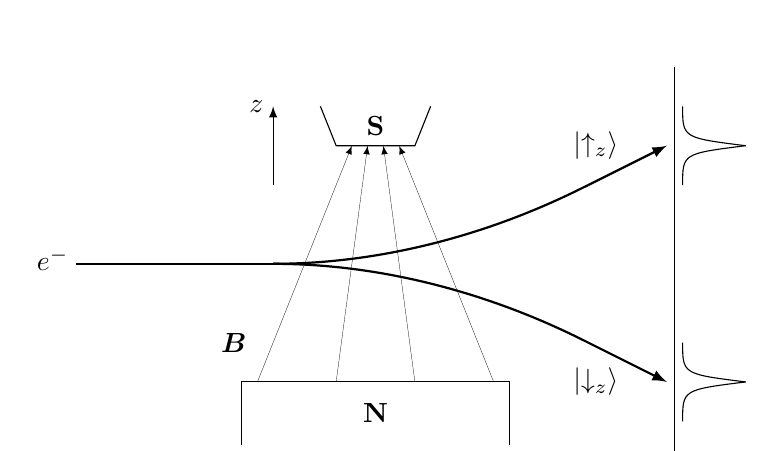
\begin{tikzpicture}
		\draw(0.6,2)--(0.8,1.5)--(1.8,1.5)--(2,2);
		\node at(1.3,1.75){\textbf S};
		\draw[ultra thin,-latex](-.2,-1.5)--(1,1.5);
		\draw[ultra thin,-latex](.8,-1.5)--(1.2,1.5);
		\draw[ultra thin,-latex](1.8,-1.5)--(1.4,1.5);
		\draw[ultra thin,-latex](2.8,-1.5)--(1.6,1.5);
		\draw(-.4,-2.3)--(-.4,-1.5)--(3,-1.5)--(3,-2.3);
		\node at(1.3,-1.9){\textbf N};
		\node at(-.5,-1){$\bm B$};
		\draw[-latex](0,1)--(0,2)node[left]{$z$};
		\node at(-2.8,.06){$e^-$};
		\draw[thick](0,0)--(-2.5,0);
		\draw[thick](0,0)parabola(4,1);
		\draw[thick,-latex](4,1)--(5,1.5);
		\node at(4.1,1.5){$\ket{\uparrow_z}$};
		\draw[thick](0,0)parabola(4,-1);
		\draw[thick,-latex](4,-1)--(5,-1.5);
		\node at(4.1,-1.5){$\ket{\downarrow_z}$};
		\draw(5.1,2.5)--(5.1,-2.5);
		\draw(5.2,1)..controls(5.2,1.4)..(6,1.5);
		\draw(5.2,2)..controls(5.2,1.6)..(6,1.5);
		\draw(5.2,-1)..controls(5.2,-1.4)..(6,-1.5);
		\draw(5.2,-2)..controls(5.2,-1.6)..(6,-1.5);
	\end{tikzpicture}
	\tikzchap Stern–Gerlach实验示意图
\end{center}
% 反常Zeeman效应。

分裂是由于粒子磁矩与磁场相互作用引起的,磁偶极矩在均匀外磁场中的势能
\[
V=-\bm\mu\cdot\bm B.
\]
在很小线度内非均匀磁场的作用下
\begin{align*}
	\bm F&=-\nabla V=\nabla(\bm\mu\cdot\bm B)\\
	&=(\bm\mu\cdot\nabla)\bm B+\cancel{(\bm B\cdot\nabla)\bm\mu}+\bm\mu\times\cancel{(\curl\bm B)}+\bm B\times\cancel{(\curl\bm\mu)},
\end{align*}
因此磁矩仅在$z$方向上受力
\[
	\bm F=0+0+\mu_z\pv{B_z}z\bm k.
\]

银原子第一激发能$\SI{10.2}\eV$,而热运动能量$\sim\kB T$
\[
T=\SI{1e5}\K,\quad \kB T=\SI{8.6}\eV
\]
一般实验条件,温度$\ll\SI{e5}\K$,银原子处于基态。只有当磁矩为量子化的(即磁矩在$z$方向的投影量子化)时,条纹才可能是分立的。

银原子在磁场中只有两个取向,有力地证明了原子在磁场中的取向是量子化的。如果角动量空间量子化理论是正确的,要得到偶数个$\mu_z$的值,唯一可能性是角量子数不是整数,而是半整数。说明电子除具有轨道角动量外还应具有自旋角动量。

\subsection{电子自旋}
\paragraph*{电子自旋假设}
\begin{compactenum}
	\item 电子不是质点,有内禀的运动——自旋。%,相应的有自旋角动量和自旋磁矩。
	\item 自旋角动量与轨道角动量类似
		\[
		\abs{\bm S}=\sqrt{s(s+1)}\hbar.
\]
		其中$s$为自旋量子数。
	\item 电子自旋角动量在空间相对外磁场的取向也是空间量子化的,
		\[
s_z=\pm\frac{\hbar}2.
\]
\end{compactenum}
\paragraph*{自旋的表达}自旋算符$\qo S$和轨道角动量算符$\qo L$具有相同形式关系
\[
	\qo S=\hat S_x\ibm i+\hat S_y\ibm j+\hat S_z\ibm k.
\]
满足角动量算符的共有性质
\begin{gather}
	\qo S\times\,\qo S=\i\hbar\qo S % ,\quad	\cmm{S_x}{S_y}=\i\hbar\hat S_z.
\end{gather}
$\{\hat S^2,\hat S_z\}$的共同本征态$\ket{s,m}$
\begin{align}
	\hat S^2\ket{s,m}&=s(s+1)\hbar^2\ket{s,m},&s&=0,\frac12,1,\frac32,\ldots\\
	\hat S_z\ket{s,m}&=m\hbar\ket{s,m},&m&=-s,-s+1,\ldots,s.
\end{align}
\paragraph*{讨论$s=1/2$}$\qo S$在任意方向上的投影只能取两个数值$\pm\hbar/2$,表象 
\[
	\ket\updownarrow\equiv\ket\pm:=\ket{\frac12,\pm\frac12}.
\]
\paragraph*{Pauli算符}定义 
\[
	\qo S=\frac\hbar{2}\qo\sigma.
\]
有对易关系
\[
	\qo\sigma\times\,\qo\sigma=2\i\qo\sigma.
\]
由$\hat S_x$等的本征值知,$\hat\sigma_x,\hat\sigma_y,\hat\sigma_z$的本征值均为$\pm 1$。

将$\hat\sigma_z\hat\sigma_x-\hat\sigma_x\hat\sigma_z=2\i\hat\sigma_y$分别左、右乘$\hat\sigma_x$,再结合$\hat\sigma_x^2=1$
\begin{align}
	\begin{cases}
		\hat\sigma_x\hat\sigma_z\hat\sigma_x-\hat\sigma_z=2\i\hat\sigma_x\hat\sigma_y\\
		\hat\sigma_z-\hat\sigma_x\hat\sigma_z\hat\sigma_x=2\i\hat\sigma_y\hat\sigma_x
	\end{cases}\thus\hat\sigma_x\hat\sigma_y=-\hat\sigma_y\hat\sigma_x=\i\hat\sigma_z.
\end{align}
或
\begin{align}
	\hat\sigma_\alpha\hat\sigma_\beta=\delta_{\alpha\beta}+\i\sum_\gamma\varepsilon_{\alpha\beta\gamma}\hat\sigma_\gamma.
\end{align}
其中$\varepsilon_{\alpha\beta\gamma}$是Levi-Civita符号。
\paragraph*{自旋算符的矩阵形式-Pauli矩阵}在$\{\hat\sigma^2,\hat\sigma_z\}$表象下
\begin{align}
	\sigma_z=\begin{bmatrix}
		1&0\\0&-1
	\end{bmatrix},
\end{align}
由$\sigma_x\dg=\sigma_x$,$\sigma_x\sigma_z=-\sigma_z\sigma_x$,可设
\[
	\begin{bmatrix}
	a&b\\b\cj&c
\end{bmatrix}\begin{bmatrix}
	1&0\\0&-1
\end{bmatrix}=-\begin{bmatrix}
	1&0\\0&-1
\end{bmatrix}\begin{bmatrix}
	a&b\\b\cj&c
\end{bmatrix},
\]
$a=c=0$,又$\sigma_x^2=1$,可取
\begin{align}
	\sigma_x=\begin{bmatrix}
		0&1\\1&0
	\end{bmatrix},
\end{align}
进而
\begin{align}
	\sigma_y=\i\sigma_x\sigma_z=\begin{bmatrix}
		0&-\i\\\i&0
	\end{bmatrix}
\end{align}
Pauli矩阵都是Hermite的、零迹的、自逆的。
\paragraph*{电子自旋态}电子的旋量波函数(spinor)
\[
	\psi(\r,t)=\begin{bmatrix}
	\psi_1(\r,t)\\\psi_2(\r,t)
\end{bmatrix}\equiv\psi_1(\r,t)\ket{\uparrow_z}+\psi_2(\r,t)\ket{\downarrow_z}.
\]
% 约定$S_z=\pm\hbar/2$的本征态对应$\zkh{1,0}\tp,\zkh{0,1}\tp$。
一般情况,自旋运动和轨道运动有相互作用,此时$\psi_1\neq\psi_2$。当自旋和轨道非耦合时,可以分离出自旋波函数$\chi(s_z)$
\[
	\psi(\r,t)=\psi_0(\r,t)\chi(s_z).
\]

\paragraph*{电子自旋磁矩}实验发现,电子自旋磁矩等于Bohr磁矩
\[
	\muB=\frac{e\hbar}{2m_\elc},\lSI
\]
则电子自旋磁矩算符
\[
	\qo{\mu_s}:=-\frac2\hbar\muB\qo S=-\frac e{m_\elc}\qo S.
\]
则
\[
	\qo{\mu_{sz}}\ket\pm=\mp\muB\ket\pm.
\]
轨道磁矩$\qo{\mu_\ell}$和自旋磁矩$\qo{\mu_s}$
\[
	\qo{\mu_\ell}=g_\ell\frac\muB\hbar\qo L,\quad\qo{\mu_s}=g_s\frac\muB\hbar\qo S,
\]
其中旋磁比$g_\ell=-1$,而$g_s=-2$,这是一种相对论效应。
\begin{example}{自旋翻转}{Spin Flip}
	处于恒稳磁场
	\[
		\bm B=B_0\zkh{\sin\theta\cos\vf,\sin\ct\cos\vf,\cos\ct}
\]
	中的电子,$t=0$时处于$\ket{\uparrow_z}$态,求$t>0$自旋翻转的概率。
	
	\textbf{解:}\quad Hamilton量
	\[
		\hat H=-\qo{\mu_s}\cdot\,\bm B=\muB\qo\sigma\cdot\,\bm B=\muB B_0\begin{bmatrix}
		\cos\ct&\sin\ct\e{-\i\vf}\\\sin\ct\e{\i\vf}&-\cos\ct
	\end{bmatrix},
\]
	易得,能量本征值$\pm\muB B_0$,及本征态
	\begin{align*}
		\ket{\uparrow_u}&=\cos\frac\ct{2}\e{-\i\vf/2}\ket{\uparrow_z}+\sin\frac\ct{2}\e{\i\vf/2}\ket{\downarrow_z},\\
		\ket{\downarrow_u}&=-\sin\frac\ct{2}\e{-\i\vf/2}\ket{\uparrow_z}+\cos\frac\ct{2}\e{\i\vf/2}\ket{\downarrow_z}.
	\end{align*}
	将待求波函数按定态展开,
	\begin{align*}
		\psi(0)&=\ket{\uparrow_z}=\cos\frac\ct{2}\e{\i\vf/2}\ket{\uparrow_u}-\sin\frac\theta{2}\e{\i\vf/2}\ket{\downarrow_u};\\
		\psi(t)&=\cos\frac\ct{2}\e{\i\vf/2}\e{-\i\muB B_0t/\hbar}\ket{\uparrow_u}-\sin\frac\theta{2}\e{\i\vf/2}\e{\i\muB B_0t/\hbar}\ket{\downarrow_u}.
	\end{align*}
	因此自旋翻转的概率
	\[
		\abs{\brkt{\downarrow_z}{\psi}}^2=\sin^2\theta\sin^2\frac{\muB B_0}\hbar t.
\]
\end{example}
\subsection{角动量算符}
若矢量算符$\qo J$满足对易关系
\[
	\qo J\times\,\qo J=\i\hbar\qo J.
\]
则称$\qo J$为角动量算符,易证,其平方算符与其分量对易
\[
	\cmm {J^2}{J_i}=0.
\]
取守恒量完全集$\{\hat J^2,\hat J_z\}$,定义升降算符
\begin{align}
	\hat J_\pm:=\hat J_x\pm\i\hat J_y.
\end{align}
注意,升降算符不是Hermite的
\[
	\hat J_\pm\dg=\hat J_\mp,
\]
因此它也不是力学量。

注意到
\begin{align*}
	\hat J_\pm\hat J_\mp&=(\hat J_x\pm\i\hat J_y)(\hat J_x\mp\i\hat J_y)\\
	&=\hat J_x^2\mp\i\cmm{J_x}{J_y}+\hat J_y^2\\
	&=\hat J_x^2+\hat J_y^2\pm\hbar\hat J_z.
\end{align*}
因此 
\begin{align}
	\hat J^2=\hat J_\pm\hat J_\mp+\hat J_z^2\mp\hbar\hat J_z.
\end{align}
\paragraph*{角动量的本征值谱}设$\{\hat J^2,\hat J_z\}$的本征态为$\ket{\lambda,m}$
\begin{align*}
	\hat J^2\ket{\lambda,m}&=\lambda\hbar^2\ket{\lambda,m},\\
	\hat J_z\ket{\lambda,m}&=m\hbar\ket{\lambda,m}.
\end{align*}

由$\cmm{J^2}{J_+}=0$,
\[
	\bra{\lambda',m'}\cmm{J^2}{J_+}\ket{\lambda,m}=(\lambda'-\lambda)\hbar^2\bra{\lambda',m'}\hat J_+\ket{\lambda,m}=0,
\]
因此,只有当$\lambda=\lambda'$时,$\bra{\lambda',m'}\hat J_+\ket{\lambda,m}$才可能不为0:
\begin{align}
	\bra{\lambda',m'}\hat J_+\ket{\lambda,m}=\vd_{\lambda\lambda'}\bra{\lambda,m'}\hat J_+\ket{\lambda,m}.
\end{align}

由$\cmm{J_z}{J_\pm}=\pm\hbar\hat J_\pm$,
\begin{align*}
	\bra{\lambda,m'}\cmm{J_z}{J_\pm}\ket{\lambda,m}&=(m'-m\mp 1)\hbar\bra{\lambda,m'}J_\pm\ket{\lambda,m}\\
	&=\pm\hbar\bra{\lambda,m'}J_\pm\ket{\lambda,m},
\end{align*}
因此$\hat J_\pm$使$m$加、减1:
\begin{align}
	\bra{\lambda',m'}\hat J_\pm\ket{\lambda,m}=\vd_{\lambda\lambda'}\vd_{m\pm 1,m'}\bra{\lambda,m\pm 1}\hat J_\pm\ket{\lambda,m}.
\end{align}

由$\cmm{J_+}{J_-}=2\hbar\hat J_z$,
\[
	\bra{\lambda,m}\cmm{J_+}{J_-}\ket{\lambda,m}=2m\hbar^2.
\]%\vd_{mm'}
插入封闭关系\footnote{下面所有$\lambda$均相同,故略去。}
\begin{align*}
	\sum_{m'}\bra{m}\hat J_+\ktbr{m'}{m'}\hat J_-\ket{m}-\bra{m}\hat J_-\ktbr{m'}{m'}\hat J_+\ket{m}=2m\hbar^2\\
	=\bra{m}\hat J_+\ktbr{m-1}{m-1}\hat J_-\ket{m}-\bra{m}\hat J_-\ktbr{m+1}{m+1}\hat J_+\ket{m}
\end{align*}
由
\[
	\bra{m-1}\hat J_-\ket{m}=\bra{m}\hat J_+\ket{m-1}\cj
\]
上式即
\begin{align}
	\abs{\bra{m}\hat J_+\ket{m-1}}^2-\abs{\bra{m-1}\hat J_+\ket{m}}^2=2m\hbar^2.
\end{align}

令$\bra{m+1}\hat J_+\ket{m}=\xi_m\hbar$,则 
\[
	\abs{\xi_{m-1}}^2-\abs{\xi_m}^2=2m.
\]
解得$\abs{\xi_m}^2=-m(m+1)+\cns.$

因为要求$\abs{\xi_m}^2\geqslant 0$,因此 
\[
m(m+1)\leqslant\cns.
\]
上式说明$m$存在一个上界$\overline m$和下界$\underline m$,使得
\begin{align*}
	\xi_{\overline m}&=\bra{\overline m+1}\hat J_+\ket{\overline m}=0;\\
	\xi_{\underline m-1}&=\bra{\underline m-1}\hat J_-\ket{\underline m}\cj=0.
\end{align*}
因此$\cns=\overline m(\overline m+1)=(\underline m-1)\underline m$,显然要求$\overline m>\underline m$,故$\overline m=-\underline m=:j$。

由于相邻的$m$相差1,故$j$只能为半整数0, \sfrac12, 1, \sfrac32, $\ldots$,且
\[
	\abs{\xi_m}^2=j(j+1)-m(m+1)=(j-m)(j+m+1).
\]

下面求$\hat J^2$的本征值,对
\[
	\hat J^2=\frac12(\hat J_+\hat J_-+\hat J_-\hat J_+)+\hat J_z^2
\]
取平均值
\[
	\lambda\hbar^2=\frac{\hbar^2}2\kh{\abs{\xi_{m-1}}^2+\abs{\xi_m}^2}+m^2\hbar^2
\]
解得$\lambda=j(j+1)$。

因此$\hat J^2,\hat J_z$是对角矩阵
\begin{align}
	\hat J^2\ket{j,m}&=j(j+1)\hbar^2\ket{j,m},&j&=0,\frac12,1,\frac32,2,\ldots\\
	\hat J_z\ket{j,m}&=m\hbar\ket{j,m},&m&=-j,-j+1,\ldots,j.
\end{align}
比如对于电子的自旋,$j=1/2,m=\pm 1/2$。

而$\hat J_\pm$的矩阵元
\begin{align}
	\hat J_\pm\ket{j,m}=\sqrt{j(j+1)-m(m\pm 1)}\ket{j,m\pm 1}.
\end{align}
\begin{example}{$\hat J_x$的平均值}{Meanvalue of Jx}
	在$\{\hat J^2,\hat J_z\}$的本征态$\ket{j,m}$上
	\begin{align*}
		\bar J_x&=\frac12(\bar J_++\bar J_-)=\frac12\bra{j,m}J_++J_-\ket{j,m}=0.\\
		\avg{J_x^2}&=\frac14\bra{j,m}J_+^2+J_+J_-+J_-J_++J_-^2\ket{j,m}.
	\end{align*}
	$\hat J_y$同理,故
	\begin{align*}
		\bar J_x=\bar J_y&=0,\\
		\avg{J_x^2}=\avg{J_y^2}&=\frac12\kh{\avg{J^2}-\avg{J_z^2}}=\frac{\hbar^2}2\fkh{\ell(\ell+1)-m^2}.
	\end{align*}
\end{example}
\begin{example}{}{}
	基底$\ket{1,-1},\ket{1,0},\ket{1,1}$,为方便略去$j\equiv 1$ %记为$\ket\upuparrows,\ket{\uparrow\downarrow},\ket\downdownarrows$
	\begin{align*}
		J_x=\begin{bmatrix}
			0&\bra{-1}\hat J_x\ket{0}&0\\
			\bra{0}\hat J_x\ket{-1}&0&\bra{0}\hat J_x\ket{1}\\
			0&\bra{1}\hat J_x\ket{0}&0
		\end{bmatrix}
	\end{align*}
	由
	\begin{align*}
		\bra{m\pm 1}\hat J_x\ket{m}&=\frac\hbar{2}\sqrt{j(j+1)-m(m\pm 1)};\\
		\bra{m\pm 1}\hat J_y\ket{m}&=\pm\frac\hbar{2\i}\sqrt{j(j+1)-m(m\pm 1)}.
	\end{align*}
	可得 
	\begin{align*}
		J_x=\frac\hbar{\sqrt2}\begin{bmatrix}
			0&1&0\\1&0&1\\0&1&0
		\end{bmatrix},\quad J_y=\frac{\i\hbar}{\sqrt2}\begin{bmatrix}
			0&1&0\\-1&0&1\\0&-1&0
		\end{bmatrix}.
	\end{align*}
\end{example}
\subsection{角动量合成}
设角动量$\qo{J_1}$和$\qo{J_2}$互相独立,也即它们的分量分别满足角动量的对易关系,而它们互相之间是对易的
\[
	\cmm{J_{1\alpha}}{J_{2\beta}}=0.
\]
则矢量和$\qo J=\qo{J_1}+\qo{J_2}$也是一个角动量算符,称为总角动量,它满足角动量的一般对易关系$\qo J\times\,\qo J=\i\hbar\qo J$。

容易看出$\hat J^2$和$\qo{J_1}$和$\qo{J_2}$并\accentd 不对易。
\paragraph*{非耦合/耦合表象}选取$\{\hat J_1^2,\hat J_{1z},\hat J_2^2,\hat J_{2z}\}$作为CSCO,基底
\[
	\ket{j_1,m_1,j_2,m_2}=\ket{j_1,m_1}\otimes\ket{j_2,m_2},
\]
即,$\qo{J_1}$只对$\ket{j_1,m_1}$作用,$\qo{J_2}$只对$\ket{j_2,m_2}$作用。这就是非耦合表象。

也可选取$\{\hat J_1^2,\hat J_2^2,\hat J^2,\hat J_z\}$作为CSCO,基底$\ket{j_1,j_2,j,m}$,这是耦合表象。

易知,表象的维数$(2j_1+1)(2j_2+1)$。
\iffalse
封闭关系
\begin{align*}
	\sum_{m_1=-j_1}^{j_1}\sum_{m_2=-j_2}^{j_2}\ktbr{j_1,m_1,j_2,m_2}{j_1,m_1,j_2,m_2}=I.
\end{align*}
\[
	\sum_{j=j_{\min}}^{j_{\max}}\sum_{m=-j}^j\ktbr{j_1,j_2,j,m}{j_1,j_2,j,m}=I.
\]
\fi

\paragraph*{非耦合/耦合表象间基底变换}对于确定的$j_1$和$j_2$,在$(2j_1+1)(2j_2+1)$维空间中
\begin{align*}
	\ket{j_1,j_2,j,m}=\sum_{m_1=-j_1}^{j_1}\sum_{m_2=-j_2}^{j_2}\ket{j_1,m_1,j_2,m_2}\bs3\brkt{j_1,m_1,j_2,m_2}{j_1,j_2,j,m},
\end{align*}
定义矢量耦合系数Clebsch-Gordan系数
\[
	\Cle_{j_1m_1j_2m_2}^{jm}=\brkt{j_1,m_1,j_2,m_2}{j_1,j_2,j,m}
\]
则
\begin{align}
	\ket{j_1,j_2,j,m}=\sum_{m_1=-j_1}^{j_1}\sum_{m_2=-j_2}^{j_2}\Cle_{j_1m_1j_2m_2}^{jm}\ket{j_1,m_1,j_2,m_2}
\end{align}
\paragraph*{总角动量本征值谱}对于确定的$j_1$和$j_2$,总角量子数$j$的取值系列为
\begin{align}
	\abs{j_1-j_2}\leqslant j\leqslant j_1+j_2
\end{align}
\prf 由$\hat J_z=\hat J_{1z}+\hat J_{2z}$
\begin{align*}
	\hat J_z\ket{j_1,j_2,j,m}=m\hbar\ket{j_1,j_2,j,m}=m\hbar\sum_{m_1,m_2}\Cle_{j_1m_1j_2m_2}^{jm}\ket{j_1,m_1,j_2,m_2};\\
	\begin{aligned}
		(\hat J_{1z}+\hat J_{2z})\ket{j_1,j_2,j,m}&=(\hat J_{1z}+\hat J_{2z})\sum_{m_1,m_2}\Cle_{j_1m_1j_2m_2}^{jm}\ket{j_1,m_1,j_2,m_2}\\
		&=(m_1+m_2)\hbar\sum_{m_1,m_2}\Cle_{j_1m_1j_2m_2}^{jm}\ket{j_1,m_1,j_2,m_2}.
	\end{aligned}
\end{align*}
由$\ket{j_1,m_1,j_2,m_2}$正交归一,
\[
m=m_1+m_2.
\]% \qed
故
\[
j_{\max}=m_{\max}=m_{1\max}+m_{2\max}=j_1+j_2,
\]
又表象变换不改变维数
\[
	\sum_{j=j_{\min}}^{j_{\max}}2j+1=(2j_1+1)(2j_2+2)\thus j_{\min}=\abs{j_1-j_2}.\rqed
\]
\paragraph*{Clebsch-Gordan系数$^\ast$}为求出Clebsch-Gordan系数,在$\ket{j_1,m_1,j_2,m_2}$基底下将$\hat J^2$对角化
\[
	\hat J^2=\hat J_1^2+\hat J_2^2+2(\hat J_{1x}\hat J_{2x}+\hat J_{1y}\hat J_{2y}+\hat J_{1z}\hat J_{2z})
\]
其中只有$\hat J_{1x}\hat J_{2x}+\hat J_{1y}\hat J_{2y}$不是对角的,可利用升降算符表示为
\[
2(\hat J_{1x}\hat J_{2x}+\hat J_{1y}\hat J_{2y})=\hat J_{1+}\hat J_{2-}+\hat J_{1-}\hat J_{2+}.
\]
因此$\hat J^2$是三对角的,
{\footnotesize
\begin{align*}
	\bra{m_1,m_2}\hat J^2\ket{m_1,m_2}&=\hbar^2\fkh{j_1(j_1+1)+j_2(j_2+1)+2m_1m_2};\\
	\bra{m_1+1,m_2-1}\hat J^2\ket{m_1,m_2}&=\hbar^2\sqrt{j_1(j_1+1)-m_1(m_1+1)}\sqrt{j_2(j_2+1)-m_2(m_2-1)};\\
	\bra{m_1-1,m_2+1}\hat J^2\ket{m_1,m_2}&=\hbar^2\sqrt{j_1(j_1+1)-m_1(m_1-1)}\sqrt{j_2(j_2+1)-m_2(m_2+1)}.
\end{align*}
}
省略了$\ket{j_1,m_1,j_2,m_2}$中的$j_1,j_2$。
\paragraph*{\Lande 因子}对于单电子原子,总角动量$\qo J=\qo L+\qo S$,则磁矩的大小
\[
	\mu=-\frac\muB\hbar\fkh{L\cos(\ell,j)+2S\cos(s,j)},\quad\muB=\frac{e\hbar}{2\mu}.
\]
由余弦定理
\begin{align*}
	\mu&=-\frac\muB\hbar\fkh{\frac{L^2+J^2-S^2}{2J}+\frac{S^2+J^2-L^2}J}\\
	&=-\frac\muB\hbar\fkh{1+\frac{J^2+S^2-L^2}{2J^2}}J.
\end{align*}
定义\Lande 因子 
\begin{align}
	g=1+\frac{j(j+1)+s(s+1)-\ell(\ell+1)}{2j(j+1)}.
\end{align}
则
\[
	\qo\mu=-\frac\muB\hbar g\qo J.
\]
\clearpage
\subsection{碱金属原子能谱的双线结构和Zeeman效应}
碱金属原子($_3$Li, $_{11}$Na等%, $_{19}$K, $_{37}$Rb, $_{55}$Cs
)中的原子实\footnote{原
子核及内层满壳电子,比如Li$^+$。}比较稳定,低激发能级来自价电子的激发。价电子的Hamilton量
\begin{align}
	\hat H_0=-\frac{\hbar^2}{2\mu}\nabla^2+V(r).
\end{align}
屏蔽Coulomb场
\[
V(r)=-\frac{e^2}r-\lambda\frac{ae^2}{r^2},\quad 0<\lambda\ll 1.
\]

非耦合表象:$\{\hat H_0,\hat L^2,\hat L_z,\hat S^2,\hat S_z\}$,有 % 能量本征值问题的解
\[
	\hat H_0\ket{n,\ell,m_\ell,m_s}=E_{n\ell}^0\ket{n,\ell,m_\ell,m_s},
\]
表达式中略去了电子自旋$s\equiv 1/2$。其简并度$2(2\ell+1)$.

耦合表象:$\{\hat H_0,\hat L^2,\hat S^2,\hat J^2,\hat J_z\}$,有 
\[
	\hat H_0\ket{n,\ell,j,m_j}=E_{n\ell}^0\ket{n,\ell,j,m_j}.
\]
\paragraph*{自旋-轨道耦合项}
除了Coulomb作用外,价电子的自旋磁矩还受到来自电子轨道运动的内磁场的作用。内磁场很强,一般$\sim10$~T。电子的自旋磁矩与内磁场的相互作用能(Thomas项)
\begin{align}
	\hat H_{LS}=\xi(r)\qo L\cdot\,\qo S%=\frac12\xi(r)\kh{\hat J^2-\hat L^2-\hat S^2}.
\end{align}
%通过繁琐的电磁学计算,或
通过Dirac方程并取非相对论极限可知
\[
	\xi(r)=\frac1{2\mu^2c^2}\frac1r\dv{V}r.
\]
$\hat H_{LS}$对能级的贡献很小,但能引起能级劈裂,形成能谱的双线结构。在原子核的壳结构中,核子之间的强自旋轨道耦合起着极其重要的作用。

将$\hat H_{LS}$改写为
\[
	\hat H_{LS}=\frac12\xi(r)\kh{\hat J^2-\hat L^2-\hat S^2}
\]
为使$\hat H=\hat H_0+\hat H_{LS}$最大限度对角化,CSCO应该包括尽量多的与$\hat H$对易的算符,由于非耦合表象中的$\hat L_z,\hat S_z$与$\hat J^2$不对易,故选取非耦合表象基底来计算$\hat H$的矩阵元。

用对角矩阵元近似代表能级
\begin{align*}
	E_{n\ell j}&\doteq\bra{n,\ell,j,m_j}\hat H\ket{n,\ell,j,m_j}\\
	&=E_{n\ell}^0+\frac{\hbar^2}2\fkh{j(j+1)-\ell(\ell+1)-\frac34}\bra{n,\ell,j,m_j}\xi(r)\ket{n,\ell,j,m_j}
\end{align*}
而
\begin{align*}
	&\bra{n,\ell,j,m_j}\xi(r)\ket{n,\ell,j,m_j}\\
	&=\sum_{s_z}\sum_{s_z'}\int\brkt{n,\ell,j,m_j}{\r,s}\bs3\bra{\r,s}\xi(r)\ket{\r',s'}\brkt{\r',s'}{n,\ell,j,m_j}\d\bm r\d\bm r'
\end{align*}
其中 
\begin{align*}
	\brkt{\r,s}{n,\ell,j,m_j}&=R_{n\ell}(r)\sum_{m_\ell,m_s}\Cle_{\ell m_\ell sm_s}^{jm_j}Y_\ell^{m_\ell}(\theta,\varphi)\chi_{m_s}(s_z);\\
	\bra{\r,s}\xi(r)\ket{\r',s'}&=\xi(r)\vd(r-r')\vd(\theta-\theta')\vd(\varphi-\varphi')\vd_{s,s'}.
\end{align*}
故
\begin{align*}
	\bra{n,\ell,j,m_j}\xi(r)\ket{n,\ell,j,m_j}&=\int\zti R_{n\ell}(r)\xi(r)R_{n\ell}(r)r^2\d r%\sum_{m_\ell m_s}\abs{\Cle_{\ell m_\ell sm_s}^{jm_j}}^2\\
	=\ave\xi_{n\ell}.
\end{align*}
计及$\hat H_{LS}$后碱金属原子的能级
\[
E_{n\ell j}\doteq E_{n\ell}^0+\frac{\hbar^2}2\fkh{j(j+1)-\ell(\ell+1)-\frac34}\ave\xi_{n\ell}
\]

$\ell\neq 0$时,$j=\ell\pm 1/2$,能级分裂为两条
\[
E_{n\ell j}\doteq E_{n\ell}^0+\hbar^2\cdot\begin{cases}
	\frac{\ell}2\ave\xi_{n\ell},& j=\ell+\frac12\\
	-\frac{\ell+1}2\ave\xi_{n\ell},& j=\ell-\frac12
\end{cases}
\]
自旋角动量和轨道角动量平行的态的能量比反平行态的能量高。

$\ell=0$时,$j=1/2$不分裂。
\paragraph*{正常Zeeman效应}1896年,Zeeman做实验发现原子在外磁场中发光谱线一分为三的现象,称为Zeeman效应。他的老师Lorentz利用电子论\footnote{用到了中学学到的Lorentz力。}对此给出了理论解释,1902年二人共同获得Nobel物理学奖。

在外磁场下价电子的Hamilton量(忽略$\hat H_{LS}$)
\[
	\hat H=\hat H_0+\frac{\muB B_0}\hbar(\hat L_z+2\hat S_z),
\]
非耦合表象中$\hat H$是对角化的,
\[
E_{n\ell m_\ell m_s}=E_{n\ell}^0+\muB B_0(m_\ell+2m_s).
\]
外磁场破坏了原子的球对称性,使能级关于磁量子数的简并完全消除。%下图表示Na黄线的正常塞曼效应,跃迁的选择定则为

跃迁的选择定则为
\[
	\D\ell=\pm 1,\quad \D m_\ell=0,\pm 1,\quad \D m_s=0.
\]
注意:跃迁只在$s=1/2$或$s=-1/2$两组能级内部进行,而不允许$s=\pm 1/2$间跃迁。
因此每条光谱线都分裂为三条,间隔相同。
\paragraph*{反常Zeeman效应}后来又发现了比三条谱线更复杂的分裂现象,称为反常Zeeman效应。这是因为在外磁场较弱时不能忽略$\hat H_{LS}$
\[
	\hat H=\hat H_0+\hat H_{LS}+\frac{\muB B_0}\hbar(\hat J_z+\hat S_z).
\]
由于$\hat J^2$与$\hat S_z$不对易,第三项矩阵元关于$j$不对角,但因磁场$B_0$较小,可取对角矩阵元近似
\[
E_{n\ell jm_j}\doteq E_{n\ell j}+\omega_\Larmor\kh{m_j\hbar+\bra{n\ell jm_j}\hat S\ket{n\ell jm_j}}
\]
换基底得
\[
	\bra{n\ell jm_j}\hat S\ket{n\ell jm_j}=\hbar\sum_{m_\ell m_s}\abs{\Cle_{\ell m_\ell sm_s}^{jm_j}}^2m_s=\hbar\sum_{m_s}\abs{\Cle_{\ell,m_\ell-m_s,sm_s}^{jm_j}}^2m_s.
\]
由
\subsection{自旋单态、三重态及纠缠态}
\paragraph*{单体近似下两个电子的自旋函数}
两电子体系,自旋自由度为2。CSCO可选择$\{\hat S_{1z},\hat S_{2z}\}$或$\{\hat S^2,\hat S_z\}$。

单体近似下,忽略两个电子间的s-s耦合。两电子的自旋函数$\chi(s_{1z},s_{2z})$是每个电子自旋函数$\chi_\alpha(s_z)$之积
\[
	\chi(s_{1z},s_{2z})=\chi_{m_s}(s_{1z})\chi_{m'_s}(s_{2z}),\quad s_1=s_2=\frac12,\quad m_s=m'_s=\pm\frac12.
\]

无耦合表象$\{\hat S_{1z},\hat S_{2z}\}$的基底$\ket{\uparrow\uparrow},\ket{\uparrow\downarrow},\ket{\downarrow\uparrow},\ket{\downarrow\downarrow}$,有对称自旋函数
\[
	\ket{\uparrow\uparrow},\ket{\downarrow\downarrow},\ket{\updownarrow}:=\frac1{\sqrt2}\kh{\ket{\uparrow\downarrow}+\ket{\downarrow\uparrow}}
\]
及反对称函数
\[
	\ket\Updownarrow :=\frac1{\sqrt2}\kh{\ket{\uparrow\downarrow}-\ket{\downarrow\uparrow}}
\]
这四个构成正交归一系。下面证明,他们是$\{\hat S^2,\hat S_z\}$的本征态。

两电子体系的总角动量平方算符
\begin{align*}
	\hat S^2=(\qo{S_1}+\qo{S_2})^2=\hat S_1^2+\hat S_2^2+2(\hat S_{1x}\hat S_{2x}+\hat S_{1y}\hat S_{2y}+\hat S_{1z}\hat S_{2z})
\end{align*}
又
\begin{gather*}
	S_z\ket\uparrow=\frac\hbar{2}\ket\uparrow,\quad S_z\ket\downarrow=\frac\hbar{2}\ket\downarrow,\\
	S_x\ket\uparrow=\frac\hbar{2}\begin{bmatrix}0&1\\1&0\end{bmatrix}\begin{bmatrix}1\\0\end{bmatrix}=\frac\hbar{2}\ket\downarrow,\quad S_x\ket\downarrow=\frac\hbar{2}\ket\uparrow\\
	S_y\ket\uparrow=\frac\hbar{2}\begin{bmatrix}0&-\i\\\i&0\end{bmatrix}\begin{bmatrix}1\\0\end{bmatrix}=\frac{\i\hbar}{2}\ket\downarrow,\quad \quad S_y\ket\downarrow=-\frac{\i\hbar}{2}\ket\uparrow.
\end{gather*}
故
\begin{align*}
	S\ket{\uparrow\uparrow}&=\frac34\hbar^2\ket{\uparrow\uparrow}+\frac34\hbar^2\ket{\uparrow\uparrow}+2\sum S_{1\alpha}\ket\uparrow S_{2\alpha}\ket\uparrow\\
	&=\kh{\frac34+\frac34+0+0+\frac12}\hbar^2\ket{\uparrow\uparrow}=2\hbar^2\ket{\uparrow\uparrow},\\
	S_z\ket{\uparrow\uparrow}&=S_{1z}\ket{\uparrow\uparrow}+S_{2z}\ket{\uparrow\uparrow}=\hbar\ket{\uparrow\uparrow}.
\end{align*}
因此四个态
\begin{align*}
	\chi_{11}&:&S^2\ket{\uparrow\uparrow}&=2\hbar^2\ket{\uparrow\uparrow}&S_z\ket{\uparrow\uparrow}&=\hbar\ket{\uparrow\uparrow}\\
	\chi_{1-1}&:&S^2\ket{\downarrow\downarrow}&=2\hbar^2\ket{\downarrow\downarrow},&S_z\ket{\downarrow\downarrow}&=-\hbar\ket{\downarrow\downarrow};\\
	\chi_{10}&:&S^2\ket\updownarrow&=2\hbar^2\ket\updownarrow,&S_z\ket\updownarrow&=0;\\
	\chi_{00}&:&S^2\ket\Updownarrow&=0,&S_z\ket\Updownarrow&=0.
\end{align*}
可作为耦合表象$\{\hat S_1^2,\hat S_2^2,\hat S^2,\hat S_z\}$的基底。
\begin{compactitem}
	\item 自旋三重态($\chi_{11},\chi_{1-1},\chi_{10}$):两电子自旋相互平行的态是三重简并的;
	\item 自旋单态($\chi_{00}$):两电子自旋相互反平行的态是单一的;
	\item 可分离态($\chi_{11},\chi_{1-1}$):由两个粒子组成的复合体系的量子态,可表示为每个粒子的量子态的乘积($\otimes$);
	\item 纠缠态($\chi_{10},\chi_{00}$):非可分离态。
\end{compactitem}
\clearpage
\section{微扰理论}
可以精确求解的量子力学问题很少,在处理各种实际问题时,除了采用适当的模型以简化问题外,往往还需要采用合适的近似解法。
\subsection{非简并定态微扰理论}
当$\hat H$比较复杂时,定态\Schr 方程不能精确求解,若$\hat H$具有以下形式
\[
	\hat H=\hat H_0+\hat H'
\]
其中$\hat H_0$是可解的,$\hat H'\ll\hat H_0$是小的修正,可令
\begin{align*}
	E_n&=E_n^{(0)}+E_n^{(1)}+E_n^{(2)}+\cdots\\
	\psi_n&=\psi_n^{(0)}+\psi_n^{(1)}+\psi_n^{(2)}+\cdots
\end{align*}
其中$E_n^{(k)}$和$\psi_n^{(k)}$与$\hat H'$的$k$次方成正比。代入原方程有
\[
	(\hat H_0+\hat H')(\psi_n^{(0)}+\psi_n^{(1)}+\cdots)=(E_n^{(0)}+E_n^{(1)}+\cdots)(\psi_n^{(0)}+\psi_n^{(1)}+\cdots)
\]
逐阶比较得到
\begin{align}
	&\text{零级方程:}&(\hat H_0-E_n^{(0)})\psi_n^{(0)}&=0;\\
	&\text{一级方程:}&(\hat H_0-E_n^{(0)})\psi_n^{(1)}&=-(\hat H'-E_n^{(1)})\psi_n^{(0)};\\
	&\text{二级方程:}&(\hat H_0-E_n^{(0)})\psi_n^{(2)}&=-(\hat H'-E_n^{(1)})\psi_n^{(1)}+E_n^{(2)}\psi_n^{(0)};\\\notag
	&\text{……}
\end{align}
一般说来,越高次的项越小,所以可以只保留最低的几阶,便有足够的精度。

以下约定:波函数的各级高级近似解与零级近似解都正交,即
\[
	\inp{\psi_n^{(0)}}{\psi_n^{(k)}}=0.
\]
对于非简并情形,即$\hat H_0$属于$E_n^{(0)}$的本征态只有一个
\[
	\psi_n^{(1)}=\sum_ma_{nm}^{(1)}\psi_m^{(0)}
\]
代入一级方程有
\[
	\sum_ma_{nm}^{(1)}(\hat H_0-E_n^{(0)})\psi_m^{(0)}=-(\hat H'-E_n^{(1)})\psi_n^{(0)}
\]
等式的两端与$\psi_k^{(0)}$内积
\[
a_{nk}^{(1)}(E_k^{(0)}-E_n^{(0)})=-\inp{\psi_k^{(0)}}{\hat H'\psi_n^{(0)}}+E_n^{(1)}\vd_{kn}
\]
取$k=n$得到一级微扰能
\begin{align}
	E_n^{(1)}=\inp{\psi_n^{(0)}}{\hat H'\psi_n^{(0)}}=:H_{nn}'
\end{align}
若取$k\neq n$,得到
\begin{align}
	a_{nk}^{(1)}=\frac{H_{kn}'}{E_k^{(0)}-E_n^{(0)}},\quad H_{kn}':=\inp{\psi_k^{(0)}}{\hat H'\psi_n^{(0)}}.
\end{align}
故一阶微扰波函数
\begin{align}
	\psi_n^{(1)}=\sum_{m\neq n}\frac{H_{mn}'}{E_m^{(0)}-E_n^{(0)}}\psi_m^{(0)}
\end{align}
微扰适用条件为
\begin{align}
	\abs{\frac{H_{mn}'}{E_m^{(0)}-E_n^{(0)}}}\ll 1.
\end{align}
\paragraph*{二阶微扰能}二级微扰方程
\[
	(\hat H_0-E_n^{(0)})\psi_n^{(2)}=-(\hat H'-E_n^{(1)})\sum_{m\neq n}\frac{H_{kn}'}{E_k^{(0)}-E_n^{(0)}}\psi_m^{(0)}+E_n^{(2)}\psi_n^{(0)}
\]
两端与$\psi_n^{(0)}$内积,得到
\begin{gather}\notag
	0=-\sum_{m\neq n}\frac{H_{mn}'}{E_k^{(0)}-E_n^{(0)}}\inp{\psi_n^{(0)}}{\hat H'\psi_m^{(0)}}+0+E_n^{(2)},\\
	\thus E_n^{(2)}=\sum_{m\neq n}\frac{\abs{H_{mn}'}^2}{E_n^{(0)}-E_m^{(0)}}.
\end{gather}

准确到二级近似下,能量的本征值为
\begin{align}
	E_n=E_n^{(0)}+H_{nn}'+\sum_{m\neq n}\frac{\abs{H_{mn}'}^2}{E_n^{(0)}-E_m^{(0)}}
\end{align}
上述理论成立需要$\hat H_0$为分离谱,无简并。
\begin{example}{电介质的极化率}{}
	各向同性的非极性分子电介质在外电场作用下极化,求感生电偶极矩。

	考虑正离子运动,无外场时为简谐运动
	\begin{gather*}
		\hat H_0=-\frac{\hbar^2}{2\mu}\dd[2]x+\frac12\mu\omega^2x^2,\\
		\hat H_n\ket n=E_n^{(0)}\ket n,\quad E_n^{(0)}=\kh{n+\frac12}\hbar\omega.
	\end{gather*}
	沿$x$向加恒定电场相当于施加微扰$\hat H'=-q\varepsilon x$
	\begin{align*}
		H_{nk}'&=\bra n\hat H'\ket k=-q\varepsilon\bra nx\ket k\\
		&=-q\varepsilon\sqrt{\frac\hbar{\mu\omega}}\kh{\sqrt{\frac{k+1}2}\vd_{n,k+1}+\sqrt{\frac k2}\vd_{n,k-1}}
	\end{align*}
	一级能量修正$H_{kk}'=0$,二阶近似能量
	\begin{align*}
		E_k&=E_k^{(0)}+0+\sum_{n\neq k}\frac{\abs{H_{nk}'}^2}{E_k^{(0)}-E_n^{(0)}}=E_k^{(0)}-\frac{q^2\varepsilon^2}{2\mu\omega^2}.
	\end{align*}
	实际上,能量是有精确解的
	\[
V=\frac12\mu\omega^2x^2-q\varepsilon x=\frac12\mu\omega^2\kh{x-\frac{q\varepsilon}{\mu\omega^2}}^2-\frac{q^2\varepsilon^2}{2\mu\omega^2}.
\]
	它的第一项只不过是把原来的谐振子势能平移了一段距离,这个移动不会影响谐振子的能级,而它的第二项正是前面求出的常数项。

	一级近似态
	\begin{align*}
		\ket{\psi_k}&=\ket k+\sum_{n\neq k}\frac{H_{nk}'}{E_k^{(0)}-E_n^{(0)}}\ket n\\
		&=\ket k+\frac{q\varepsilon}{\sqrt{\hbar\mu\omega^3}}\kh{\sqrt{\frac{k+1}2}\ket{k+1}-\sqrt{\frac k2}\ket{k-1}},
	\end{align*}
	无外加场时,非极性分子正(负)离子的位置平均值$\bra kx\ket k=0$,即固有电偶极矩为零,而加外电场后正离子位移
	\[
		\bra{\psi_k}x\ket{\psi_k}=\frac{2q\varepsilon}{\sqrt{\hbar\mu\omega^3}}\kh{\sqrt{\frac{k+1}2}\brkt k{k+1}-\sqrt{\frac k2}\brkt k{k-1}}=\frac{q\varepsilon}{\mu\omega^2}.
\]
	故感生电偶极矩$D$和极化率$\kappa$
	\[
D=\abs q\frac{2\abs q\varepsilon}{\mu\omega^2}=\frac{2q^2\varepsilon}{\mu\omega^2},\quad \kappa=\frac D\varepsilon=\frac{2q^2}{\mu\omega^2}.
\]
\end{example}
\begin{example}{氦原子}{}
	氦原子在原子核外有两个电子,Hamilton量包括两个电子在原子核的Column引力场中的运动
	\[
		\hat H_0=\kh{-\frac12\nabla_1^2-\frac Z{r_1}}+\kh{-\frac12\nabla_1^2-\frac Z{r_2}};
\]
	以及两个电子之间的Column排斥能(微扰项)
	\[
		\hat H'=\frac1{r_{12}}.
\]

	它对于两个电子空间坐标的交换是对称的。由于电子是Fermi子,两个电子相应的自旋态只能反对称的自旋单态$\chi_{00}$
	\[
		\psi(\r_1,\r_2)=\psi_{100}(\r_1)\psi_{100}(\r_2)\chi_{00}(s_{1z},s_{2z}).
\]
	相应的本征值$E_1^0=-Z^2$,一级修正
	\[
		\ave{\frac1{r_{12}}}=\int\frac{\abs{\psi_{100}(\r_1)\psi_{100}(\r_2)}^2}{r_{12}}\d\r_1\nd\r_2.
\]
	由
	\[
		\psi_{100}(\r)=\frac{Z^{3/2}}{\sqrt\pi}\e{-Zr};\quad \int\frac{\e{-Z(r_1+r_2)}}{r_{12}}\d\r_1\nd\r_2=\frac{5\pi^2}{8Z^5}.
\]
	得
	\[
E=-Z^2+\frac58Z.
\]
\end{example}
\subsection{简并定态微扰理论}
实际问题中,特别是处理体系的激发态时,常常碰到简并态或近似简并态。此时,非简并态微扰论是不适用的。

这里首先碰到的困难是:零级能量给定后,对应的零级波函数并未确定,这是简并态微扰论首先要解决的问题。

体系能级的简并性与体系的对称性密切相关。当考虑微扰之后,如体系的某种对称性受到破坏,则能级可能分裂,简并将部分或全部解除。因而在简并态微扰中,充分考虑体系的对称性及其破缺是至关重要的。
\paragraph*{一级微扰能和零级波函数}$E_n^{(0)}$简并时,
\[
	\hat H^{(0)}\psi_{ni}^{(0)}=E_n^{(0)}\psi_{ni}^{(0)},\quad (i=1,2,\ldots,k).
\]
简并度$f_n=k$,引入微扰后假设
\[
	\psi_n^{(0)}=\sum_{i=1}^kc_i^{(0)}\psi_{ni}^{(0)}.
\]
代入一级微扰方程
\[
	(\hat H_0-E_n^{(0)})\psi_n^{(1)}=-(\hat H'-E_n^{(1)})\sum_{i=1}^kc_i^{(0)}\psi_{ni}^{(0)}.
\]
两端与$\psi_{nj}^{(0)}$内积
\[
0=-\sum_{k=1}^nc_i^{(0)}\fkh{\inp{\psi_{nj}^{(0)}}{\hat H'\psi_{ni}^{(0)}}-E_n^{(1)}\vd_{ij}}.
\]
记
\begin{align}
	H_{ji}':=\inp{\psi_{nj}^{(0)}}{\hat H'\psi_{ni}^{(0)}}
\end{align}
得到久期(secular)方程
\begin{align}
	\det(H'-E_n^{(1)}I)=\begin{vmatrix}
		H_{11}'-E_n^{(1)}&H_{12}'&\cdots&H_{1k}'\\
		H_{21}'&H_{22}'-E_n^{(1)}&\cdots&H_{2k}'\\
		\vdots&\vdots&\ddots&\vdots\\
		H_{k1}'&H_{k2}'&\cdots&H_{kk}'-E_n^{(1)}
	\end{vmatrix}=0.
\end{align}
从中可以解出$E_n^{(1)}$以及它们对应的$c_i^{(0)}$,这就决定了一级微扰能和零级波函数。
\paragraph*{Stark效应}Stark效应就是原子或分子在外电场作用下能级和光谱发生分裂的现象。
\subsectionstar{变分法}没讲
\clearpage
\section{跃迁理论}
若体系的Hamilton量$\hat H_0$不显含时间,能量本征值问题的解为
\[
	\hat H_0\ket n=E_n\ket n.
\]
若$\hat H(t)=\hat H_0+\hat H'(t)$显含时间,体系将有一定的概率离开初态$\ket{k}$而处于其它定态$\ket{k'}$,这就是\textbf{量子跃迁}。
\subsection{量子态随时间的变化}
状态随时间的演化由\Schr 方程决定
\begin{align}
	\begin{cases}
		\i\hbar\pp t\ket{\psi(t)}=\hat H(t)\ket{\psi(t)},\\
		\ket{\psi(0)}=\ket{k}.
	\end{cases}
\end{align}
采用能量$\hat H_0$表象 
\begin{align}
	\ket{\psi(0)}=\sum_n C_{nk}(t)\ket n\e{-\i E_nt/\hbar},\quad C_{nk}(0)=\vd_{nk}.
\end{align}
体系$t$时刻跃迁到定态$\ket{k'}$的概率为$\abs{C_{k'k}(t)}^2$。

为求出跃迁概率,将表象表达式带入\Schr 方程,假定$\hat H'$中不包括$\p/\p t$作用
{\small\begin{align}\notag
	\i\hbar\sum_n\fkh{\dot C_{nk}(t)-\cancel{\frac{\i E_nC_{nk}(t)}\hbar}}\ket n\e{-\i E_nt/\hbar}&=\sum_nC_{nk}(t)\fkh{\cancel{E_n}+\hat H'(t)}\ket n\e{-\i E_nt/\hbar}.\\
	\i\hbar\sum_n\dot C_{nk}(t)\ket n\e{-\i E_nt/\hbar}&=\sum_nC_{nk}(t)\hat H'(t)\ket n\e{-\i E_nt/\hbar}.
\end{align}}
与$\ket{k'}$内积
\begin{align}
	\i\hbar\dot C_{k'k}(t)\e{-\i E_{k'}t/\hbar}=\sum_nC_{nk}(t)\bra{k'}\hat H'(t)\ket n\e{-\i E_nt/\hbar}
\end{align}
定义 
\begin{align}
	H_{k'n}'(t):=\bra{k'}\hat H'(t)\ket n,\quad\omega_{k'n}=\frac{E_{k'}-E_n}\hbar.
\end{align}
得到跃迁振幅$C_{k'k}(t)$满足 
\begin{align}
	\begin{cases}
		\i\hbar\dd tC_{k'k}(t)=\sum_nH'_{k'n}(t)\e{\i\omega_{k'n}t}C_{nk}(t),\\
		C_{k'k}(0)=\vd_{k'k}.
	\end{cases}
\end{align}
两边对$t$积分
\begin{align}
	C_{k'k}(t)=C_{k'k}(0)+\frac1{\i\hbar}\int_0^t\sum_nH'_{k'n}(\tau)\e{\i\omega_{k'n}\tau}C_{nk}(\tau)\d\tau
\end{align}
这是一个积分方程,可采用迭代求解。

迭代一次
\begin{align*}
	C_{k'k}(t)&=\vd_{k'k}+\frac1{\i\hbar}\int_0^t\sum_nH'_{k'n}(\tau)\e{\i\omega_{k'n}\tau}\cdot\\
	&\quad\fkh{\vd_{nk}+\frac1{\i\hbar}\int_0^\tau\sum_nH'_{k'n}(\pi)\e{\i\omega_{k'n}\pi}C_{nk}(\pi)\d\pi}\d\tau\\
	&=\vd_{k'k}+\frac1{\i\hbar}\int_0^tH'_{k'k}(\tau)\e{\i\omega_{k'k}\tau}\d\tau+\cdots
\end{align*}
零级近似
\[
C_{k'k}^{(0)}=\vd_{k'k};
\]
一级近似 
\[
C_{k'k}^{(1)}=\frac1{\i\hbar}\int_0^tH'_{k'k}(\tau)\e{\i\omega_{k'k}\tau}\d\tau,
\]
代表直接从初态$\ket k$跃迁到末态$\ket{k'}$,故跃迁概率
\begin{align}
	P_{k'k}(t)=\frac1{\hbar^2}\abs{\int_0^tH'_{k'k}(\tau)\e{\i\omega_{k'k}\tau}\d\tau}^2.
\end{align}
由$\hat H'$是Hermite的。故$P_{k'k}=P_{kk'}$,即从初态到末态的跃迁概率等于从末态到初态的跃迁概率。

对于初态$\ket k$和末态$\ket{k'}$都有简并的情况,计算跃迁概率应对$\ket k$能级各简并态求平均,而对$\ket{k'}$能级各简并态求和,此时跃迁概率不一定相等。

二级近似
\[
C_{k'k}^{(2)}=\frac1{(\i\hbar)^2}\sum_n\int_0^tH'_{k'n}(\tau)\e{\i\omega_{k'n}\tau}\int_0^\tau H'_{nk}(\pi)\e{\i\omega_{nk}\pi}\d\pi\d\tau,
\]
代表从初态$\ket k$经中间态$\ket n$跃迁到末态$\ket{k'}$。
\subsectionstar{周期微扰和常微扰}
没讲
\subsection{光的吸收与辐射}
光与原子的相互作用包括受激吸收、受激辐射和自发辐射。其中自发辐射是前面的理论无法解释的,Einstein基于热力学和统计物理中的平衡概念给出过半唯象的理论,巧妙地导出了自发辐射系数。
\paragraph*{电偶极跃迁}若入射光为理想单色偏振光,
\[
	\bm E=\bm E_0\cos(\omega t-\bm k\cdot\bm r),\quad\bm B=\frac{\bm k}{\abs k}\times\bm E.\CGS
\]
对电子的作用 
\[
	\bm f=-e\kh{\bm E+\frac{\bm v}c\times\bm B},\CGS
\]
原子中电子的速度$v\ll c$,故可仅考虑电场的作用。

对于可见光和紫外光\footnote{X光并不满足。}波长$\lambda\gg a$\,(Bohr半径),故在原子范围内电场可视为均匀场
\[
	\bm E\doteq\bm E_0\cos\omega t.
\]
光对原子的作用可近似表示成电子的电偶极矩与电场的相互作用
\[
	\hat H'(t)=-\bm D\cdot\bm E=W\cos\omega t.
\]
其中电子的电偶极矩$\bm D=-e\r$,电偶极矩与电场作用引起的跃迁称为电偶极跃迁。
\begin{align*}
	C_{k'k}^{(1)}(t)&=\frac1{\i\hbar}\int_0^tH_{k'k}'(\tau)\e{-\i\omega_{k'k}\tau}\d\tau=\frac{W_{k'k}}{\i\hbar}\int_0^t\cos\omega\tau\e{-i\omega_{k'k}\tau}\d\tau\\
	&=-\frac{W_{k'k}}{2\hbar}\fkh{\frac{\e{\i(\omega_{k'k}+\omega)t}-1}{\omega_{k'k}+\omega}+\frac{\e{\i(\omega_{k'k}-\omega)t}-1}{\omega_{k'k}-\omega}}.
\end{align*}
下面讨论原子吸收光的跃迁,$E_{k'}>E_k$,只有当入射光$\omega\doteq\omega_{k'k}$时,才会引起$E_k\to E_{k'}$跃迁,此时
\begin{align*}
	C_{k'k}^{(1)}(t)=-\frac{W_{k'k}}{2\hbar}\frac{\e{\i(\omega_{k'k}-\omega)t}-1}{\omega_{k'k}-\omega}.
\end{align*}
从$k\to k'$的概率为
\begin{align}
	P_{k'k}(t)=\abs{C_{k'k}^{(1)}(t)}^2=\frac{\abs{W_{k'k}}^2}{4\hbar^2}\fkh{\frac{\sin(\omega_{k'k}-\omega)t/2}{(\omega_{k'k}-\omega)/2}}^2
\end{align}
$t\to\infty$时,有 
\begin{align}
	P_{k'k}(t)=\frac{\pi t}{2\hbar^2}\abs{W_{k'k}}^2\vd\kh{\omega_{k'k}-\omega};
\end{align}
跃迁速率
\begin{align}
	w_{k'k}&=\dd tP_{k'k}=\frac\pi{2\hbar^2}\abs{W_{k'k}}^2\vd\kh{\omega_{k'k}-\omega}\\
	&=\frac\pi{2\hbar^2}\abs{\bm D_{k'k}}^2E_0^2\cos^2\theta\vd\kh{\omega_{k'k}-\omega},
\end{align}
$\theta$为电子的电偶极矩与电场的夹角。

而对于非偏振光,应对$\cos^2\theta$取平均
\[
	\ave{\cos^2\theta}=\frac1{4\pi}\int_0^{2\pi}\bs5\int_0^\pi\cos^2\theta\sin\theta\d\theta\nd\phi=\frac13.
\]
跃迁速率 
\begin{align}
	w_{k'k}=\frac\pi{6\hbar^2}\abs{\bm D_{k'k}}^2E_0^2\vd\kh{\omega_{k'k}-\omega}.
\end{align}

对于非单色光,总跃迁速率是对各种频率求和
\begin{align}
	w\tot=\int\iti\omega_{k'k}\d\omega=\frac\pi{6\hbar^2}\abs{\bm D_{k'k}}^2E_0^2(\omega_{k'k}).
\end{align}

频率为$\omega$的电磁波能量密度的时间平均值
\begin{align*}
	\rho(\omega)=\frac1{8\pi}\ave{E^2+B^2}=\frac1{8\pi}E_0^2(\omega).\CGS
\end{align*}
故非偏振自然光引起的跃迁速率
\begin{align}
	w_{k'k}=\frac{4\pi^2}{3\hbar^2}\abs{\bm D_{k'k}}^2\rho(\omega_{k'k})=\frac{4\pi^2e^2}{3\hbar^2}\abs{\r_{k'k}}^2\rho(\omega_{k'k}).
\end{align}
由$\r$为奇宇称算符,只有$\ket k,\ket{k'}$宇称相反时,$\abs{\r_{k'k}}^2$才不为0。又
\begin{align*}
	\r=r\zkh{\sin\theta\cos\vf,\sin\theta\sin\vf,\cos\ct}
\end{align*}
由第 \pageref{costhetaYlm} 页的球谐函数递推式知,跃迁态间需满足$\D\ell=\pm 1,\,\D m=0,\pm 1$。
\paragraph*{Einstein跃迁理论}
\end{document}